\begin{figure}[H] \centering % Created by tikzDevice version 0.12.4 on 2023-07-25 11:08:58
% !TEX encoding = UTF-8 Unicode
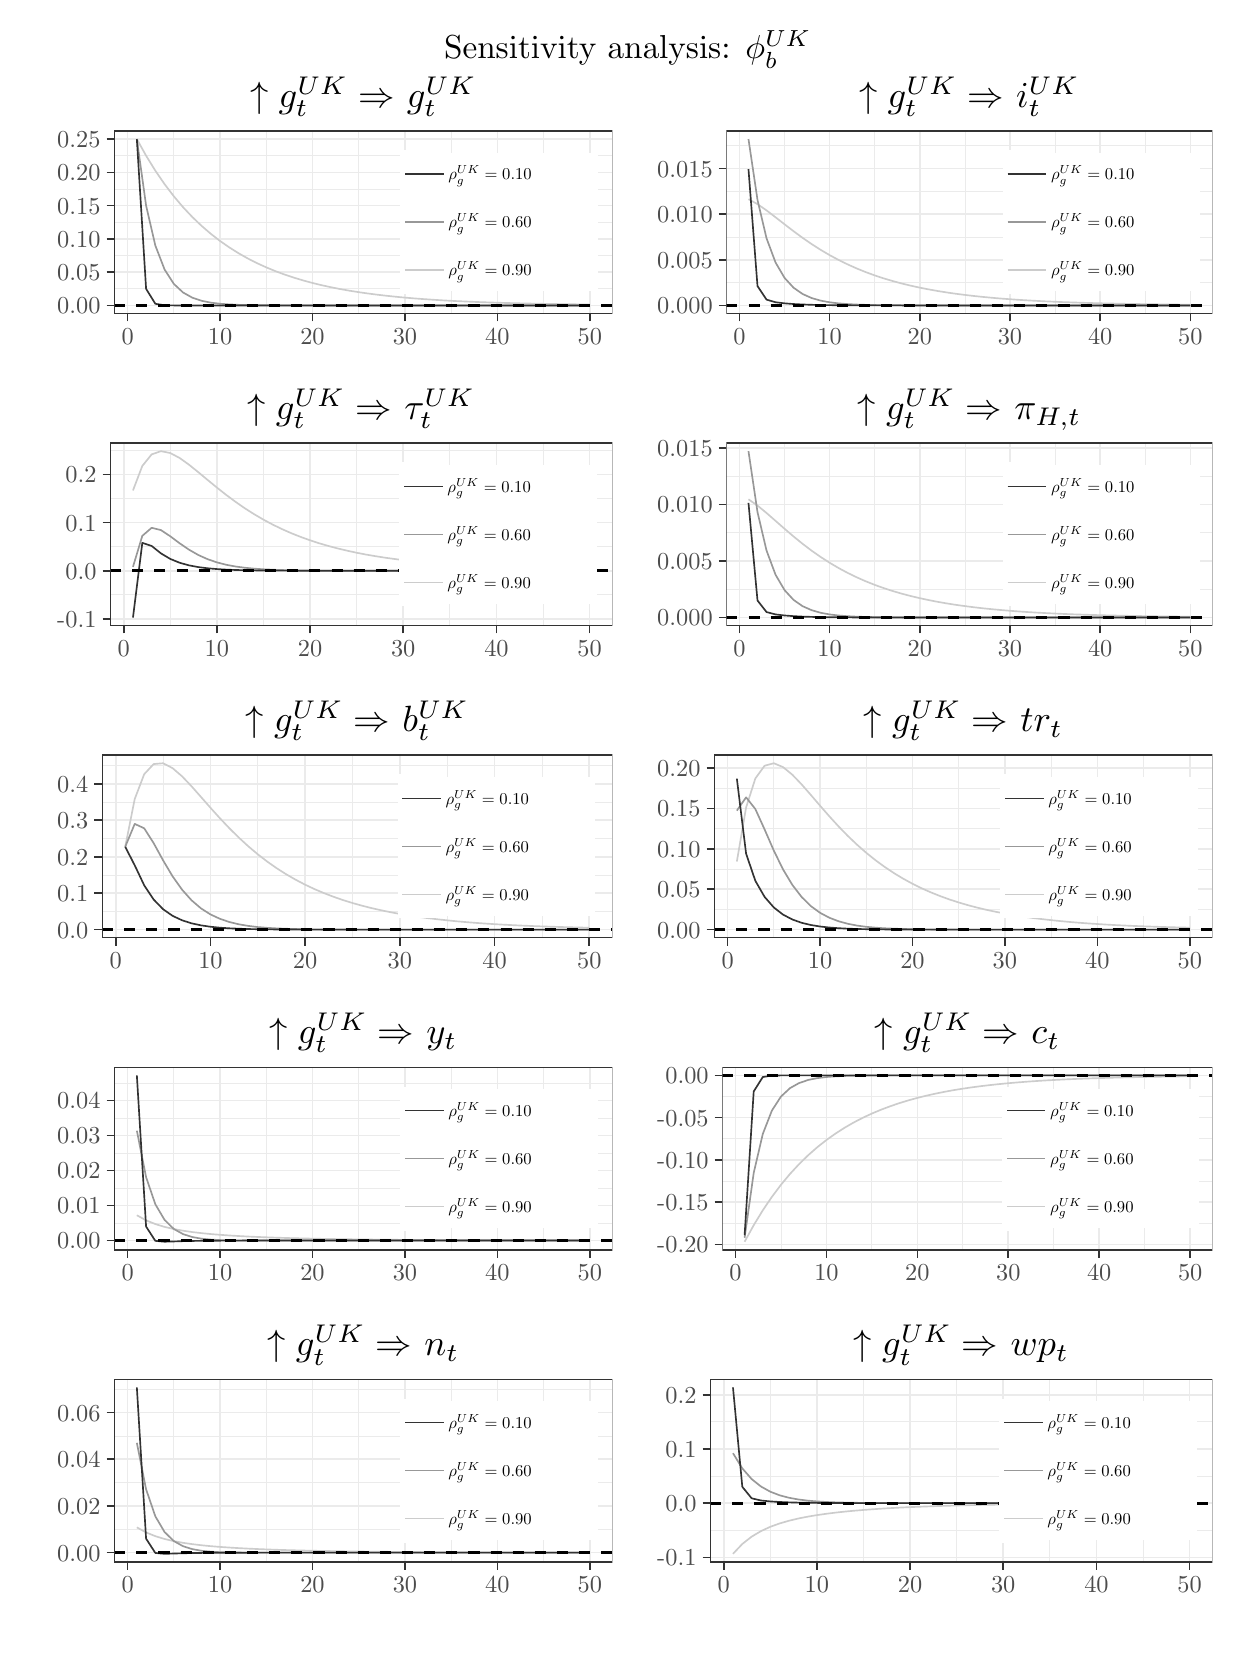
\begin{tikzpicture}[x=1pt,y=1pt]
\definecolor{fillColor}{RGB}{255,255,255}
\path[use as bounding box,fill=fillColor,fill opacity=0.00] (0,0) rectangle (433.62,578.16);
\begin{scope}
\path[clip] (  0.00,451.10) rectangle (216.81,563.87);
\definecolor{drawColor}{RGB}{255,255,255}
\definecolor{fillColor}{RGB}{255,255,255}

\path[draw=drawColor,line width= 0.6pt,line join=round,line cap=round,fill=fillColor] (  0.00,451.10) rectangle (216.81,563.87);
\end{scope}
\begin{scope}
\path[clip] ( 31.27,474.78) rectangle (211.31,540.91);
\definecolor{fillColor}{RGB}{255,255,255}

\path[fill=fillColor] ( 31.27,474.78) rectangle (211.31,540.91);
\definecolor{drawColor}{gray}{0.92}

\path[draw=drawColor,line width= 0.3pt,line join=round] ( 31.27,483.79) --
	(211.31,483.79);

\path[draw=drawColor,line width= 0.3pt,line join=round] ( 31.27,495.82) --
	(211.31,495.82);

\path[draw=drawColor,line width= 0.3pt,line join=round] ( 31.27,507.84) --
	(211.31,507.84);

\path[draw=drawColor,line width= 0.3pt,line join=round] ( 31.27,519.87) --
	(211.31,519.87);

\path[draw=drawColor,line width= 0.3pt,line join=round] ( 31.27,531.89) --
	(211.31,531.89);

\path[draw=drawColor,line width= 0.3pt,line join=round] ( 52.81,474.78) --
	( 52.81,540.91);

\path[draw=drawColor,line width= 0.3pt,line join=round] ( 86.22,474.78) --
	( 86.22,540.91);

\path[draw=drawColor,line width= 0.3pt,line join=round] (119.62,474.78) --
	(119.62,540.91);

\path[draw=drawColor,line width= 0.3pt,line join=round] (153.02,474.78) --
	(153.02,540.91);

\path[draw=drawColor,line width= 0.3pt,line join=round] (186.43,474.78) --
	(186.43,540.91);

\path[draw=drawColor,line width= 0.6pt,line join=round] ( 31.27,477.78) --
	(211.31,477.78);

\path[draw=drawColor,line width= 0.6pt,line join=round] ( 31.27,489.81) --
	(211.31,489.81);

\path[draw=drawColor,line width= 0.6pt,line join=round] ( 31.27,501.83) --
	(211.31,501.83);

\path[draw=drawColor,line width= 0.6pt,line join=round] ( 31.27,513.86) --
	(211.31,513.86);

\path[draw=drawColor,line width= 0.6pt,line join=round] ( 31.27,525.88) --
	(211.31,525.88);

\path[draw=drawColor,line width= 0.6pt,line join=round] ( 31.27,537.90) --
	(211.31,537.90);

\path[draw=drawColor,line width= 0.6pt,line join=round] ( 36.11,474.78) --
	( 36.11,540.91);

\path[draw=drawColor,line width= 0.6pt,line join=round] ( 69.52,474.78) --
	( 69.52,540.91);

\path[draw=drawColor,line width= 0.6pt,line join=round] (102.92,474.78) --
	(102.92,540.91);

\path[draw=drawColor,line width= 0.6pt,line join=round] (136.32,474.78) --
	(136.32,540.91);

\path[draw=drawColor,line width= 0.6pt,line join=round] (169.72,474.78) --
	(169.72,540.91);

\path[draw=drawColor,line width= 0.6pt,line join=round] (203.13,474.78) --
	(203.13,540.91);
\definecolor{drawColor}{gray}{0.80}

\path[draw=drawColor,line width= 0.6pt,line join=round] ( 39.45,537.90) --
	( 42.79,531.89) --
	( 46.13,526.48) --
	( 49.47,521.61) --
	( 52.81,517.23) --
	( 56.15,513.28) --
	( 59.50,509.73) --
	( 62.84,506.54) --
	( 66.18,503.66) --
	( 69.52,501.07) --
	( 72.86,498.75) --
	( 76.20,496.65) --
	( 79.54,494.76) --
	( 82.88,493.06) --
	( 86.22,491.54) --
	( 89.56,490.16) --
	( 92.90,488.92) --
	( 96.24,487.81) --
	( 99.58,486.81) --
	(102.92,485.90) --
	(106.26,485.09) --
	(109.60,484.36) --
	(112.94,483.70) --
	(116.28,483.11) --
	(119.62,482.58) --
	(122.96,482.10) --
	(126.30,481.67) --
	(129.64,481.28) --
	(132.98,480.93) --
	(136.32,480.61) --
	(139.66,480.33) --
	(143.00,480.08) --
	(146.34,479.85) --
	(149.68,479.64) --
	(153.02,479.45) --
	(156.36,479.29) --
	(159.70,479.14) --
	(163.04,479.00) --
	(166.38,478.88) --
	(169.72,478.77) --
	(173.06,478.67) --
	(176.40,478.58) --
	(179.74,478.50) --
	(183.08,478.43) --
	(186.43,478.36) --
	(189.77,478.31) --
	(193.11,478.25) --
	(196.45,478.21) --
	(199.79,478.16) --
	(203.13,478.13);
\definecolor{drawColor}{RGB}{152,152,152}

\path[draw=drawColor,line width= 0.6pt,line join=round] ( 39.45,537.90) --
	( 42.79,513.86) --
	( 46.13,499.43) --
	( 49.47,490.77) --
	( 52.81,485.57) --
	( 56.15,482.46) --
	( 59.50,480.59) --
	( 62.84,479.46) --
	( 66.18,478.79) --
	( 69.52,478.39) --
	( 72.86,478.15) --
	( 76.20,478.00) --
	( 79.54,477.91) --
	( 82.88,477.86) --
	( 86.22,477.83) --
	( 89.56,477.81) --
	( 92.90,477.80) --
	( 96.24,477.79) --
	( 99.58,477.79) --
	(102.92,477.79) --
	(106.26,477.78) --
	(109.60,477.78) --
	(112.94,477.78) --
	(116.28,477.78) --
	(119.62,477.78) --
	(122.96,477.78) --
	(126.30,477.78) --
	(129.64,477.78) --
	(132.98,477.78) --
	(136.32,477.78) --
	(139.66,477.78) --
	(143.00,477.78) --
	(146.34,477.78) --
	(149.68,477.78) --
	(153.02,477.78) --
	(156.36,477.78) --
	(159.70,477.78) --
	(163.04,477.78) --
	(166.38,477.78) --
	(169.72,477.78) --
	(173.06,477.78) --
	(176.40,477.78) --
	(179.74,477.78) --
	(183.08,477.78) --
	(186.43,477.78) --
	(189.77,477.78) --
	(193.11,477.78) --
	(196.45,477.78) --
	(199.79,477.78) --
	(203.13,477.78);
\definecolor{drawColor}{gray}{0.20}

\path[draw=drawColor,line width= 0.6pt,line join=round] ( 39.45,537.90) --
	( 42.79,483.79) --
	( 46.13,478.38) --
	( 49.47,477.84) --
	( 52.81,477.79) --
	( 56.15,477.78) --
	( 59.50,477.78) --
	( 62.84,477.78) --
	( 66.18,477.78) --
	( 69.52,477.78) --
	( 72.86,477.78) --
	( 76.20,477.78) --
	( 79.54,477.78) --
	( 82.88,477.78) --
	( 86.22,477.78) --
	( 89.56,477.78) --
	( 92.90,477.78) --
	( 96.24,477.78) --
	( 99.58,477.78) --
	(102.92,477.78) --
	(106.26,477.78) --
	(109.60,477.78) --
	(112.94,477.78) --
	(116.28,477.78) --
	(119.62,477.78) --
	(122.96,477.78) --
	(126.30,477.78) --
	(129.64,477.78) --
	(132.98,477.78) --
	(136.32,477.78) --
	(139.66,477.78) --
	(143.00,477.78) --
	(146.34,477.78) --
	(149.68,477.78) --
	(153.02,477.78) --
	(156.36,477.78) --
	(159.70,477.78) --
	(163.04,477.78) --
	(166.38,477.78) --
	(169.72,477.78) --
	(173.06,477.78) --
	(176.40,477.78) --
	(179.74,477.78) --
	(183.08,477.78) --
	(186.43,477.78) --
	(189.77,477.78) --
	(193.11,477.78) --
	(196.45,477.78) --
	(199.79,477.78) --
	(203.13,477.78);
\definecolor{drawColor}{RGB}{0,0,0}

\path[draw=drawColor,line width= 1.1pt,dash pattern=on 4pt off 4pt ,line join=round] ( 31.27,477.78) -- (211.31,477.78);
\definecolor{drawColor}{gray}{0.20}

\path[draw=drawColor,line width= 0.6pt,line join=round,line cap=round] ( 31.27,474.78) rectangle (211.31,540.91);
\end{scope}
\begin{scope}
\path[clip] (  0.00,  0.00) rectangle (433.62,578.16);
\definecolor{drawColor}{gray}{0.30}

\node[text=drawColor,anchor=base east,inner sep=0pt, outer sep=0pt, scale=  0.88] at ( 26.32,474.75) {0.00};

\node[text=drawColor,anchor=base east,inner sep=0pt, outer sep=0pt, scale=  0.88] at ( 26.32,486.78) {0.05};

\node[text=drawColor,anchor=base east,inner sep=0pt, outer sep=0pt, scale=  0.88] at ( 26.32,498.80) {0.10};

\node[text=drawColor,anchor=base east,inner sep=0pt, outer sep=0pt, scale=  0.88] at ( 26.32,510.83) {0.15};

\node[text=drawColor,anchor=base east,inner sep=0pt, outer sep=0pt, scale=  0.88] at ( 26.32,522.85) {0.20};

\node[text=drawColor,anchor=base east,inner sep=0pt, outer sep=0pt, scale=  0.88] at ( 26.32,534.87) {0.25};
\end{scope}
\begin{scope}
\path[clip] (  0.00,  0.00) rectangle (433.62,578.16);
\definecolor{drawColor}{gray}{0.20}

\path[draw=drawColor,line width= 0.6pt,line join=round] ( 28.52,477.78) --
	( 31.27,477.78);

\path[draw=drawColor,line width= 0.6pt,line join=round] ( 28.52,489.81) --
	( 31.27,489.81);

\path[draw=drawColor,line width= 0.6pt,line join=round] ( 28.52,501.83) --
	( 31.27,501.83);

\path[draw=drawColor,line width= 0.6pt,line join=round] ( 28.52,513.86) --
	( 31.27,513.86);

\path[draw=drawColor,line width= 0.6pt,line join=round] ( 28.52,525.88) --
	( 31.27,525.88);

\path[draw=drawColor,line width= 0.6pt,line join=round] ( 28.52,537.90) --
	( 31.27,537.90);
\end{scope}
\begin{scope}
\path[clip] (  0.00,  0.00) rectangle (433.62,578.16);
\definecolor{drawColor}{gray}{0.20}

\path[draw=drawColor,line width= 0.6pt,line join=round] ( 36.11,472.03) --
	( 36.11,474.78);

\path[draw=drawColor,line width= 0.6pt,line join=round] ( 69.52,472.03) --
	( 69.52,474.78);

\path[draw=drawColor,line width= 0.6pt,line join=round] (102.92,472.03) --
	(102.92,474.78);

\path[draw=drawColor,line width= 0.6pt,line join=round] (136.32,472.03) --
	(136.32,474.78);

\path[draw=drawColor,line width= 0.6pt,line join=round] (169.72,472.03) --
	(169.72,474.78);

\path[draw=drawColor,line width= 0.6pt,line join=round] (203.13,472.03) --
	(203.13,474.78);
\end{scope}
\begin{scope}
\path[clip] (  0.00,  0.00) rectangle (433.62,578.16);
\definecolor{drawColor}{gray}{0.30}

\node[text=drawColor,anchor=base,inner sep=0pt, outer sep=0pt, scale=  0.88] at ( 36.11,463.76) {0};

\node[text=drawColor,anchor=base,inner sep=0pt, outer sep=0pt, scale=  0.88] at ( 69.52,463.76) {10};

\node[text=drawColor,anchor=base,inner sep=0pt, outer sep=0pt, scale=  0.88] at (102.92,463.76) {20};

\node[text=drawColor,anchor=base,inner sep=0pt, outer sep=0pt, scale=  0.88] at (136.32,463.76) {30};

\node[text=drawColor,anchor=base,inner sep=0pt, outer sep=0pt, scale=  0.88] at (169.72,463.76) {40};

\node[text=drawColor,anchor=base,inner sep=0pt, outer sep=0pt, scale=  0.88] at (203.13,463.76) {50};
\end{scope}
\begin{scope}
\path[clip] (  0.00,  0.00) rectangle (433.62,578.16);
\definecolor{fillColor}{RGB}{255,255,255}

\path[fill=fillColor] (135.68,482.83) rectangle (205.92,532.86);
\end{scope}
\begin{scope}
\path[clip] (  0.00,  0.00) rectangle (433.62,578.16);
\definecolor{fillColor}{RGB}{255,255,255}

\path[fill=fillColor] (134.68,516.52) rectangle (152.03,533.86);
\end{scope}
\begin{scope}
\path[clip] (  0.00,  0.00) rectangle (433.62,578.16);
\definecolor{drawColor}{gray}{0.20}

\path[draw=drawColor,line width= 0.6pt,line join=round] (136.42,525.19) -- (150.29,525.19);
\end{scope}
\begin{scope}
\path[clip] (  0.00,  0.00) rectangle (433.62,578.16);
\definecolor{drawColor}{gray}{0.20}

\path[draw=drawColor,line width= 0.6pt,line join=round] (136.42,525.19) -- (150.29,525.19);
\end{scope}
\begin{scope}
\path[clip] (  0.00,  0.00) rectangle (433.62,578.16);
\definecolor{drawColor}{gray}{0.20}

\path[draw=drawColor,line width= 0.6pt,line join=round] (136.42,525.19) -- (150.29,525.19);
\end{scope}
\begin{scope}
\path[clip] (  0.00,  0.00) rectangle (433.62,578.16);
\definecolor{fillColor}{RGB}{255,255,255}

\path[fill=fillColor] (134.68,499.17) rectangle (152.03,516.52);
\end{scope}
\begin{scope}
\path[clip] (  0.00,  0.00) rectangle (433.62,578.16);
\definecolor{drawColor}{RGB}{152,152,152}

\path[draw=drawColor,line width= 0.6pt,line join=round] (136.42,507.84) -- (150.29,507.84);
\end{scope}
\begin{scope}
\path[clip] (  0.00,  0.00) rectangle (433.62,578.16);
\definecolor{drawColor}{RGB}{152,152,152}

\path[draw=drawColor,line width= 0.6pt,line join=round] (136.42,507.84) -- (150.29,507.84);
\end{scope}
\begin{scope}
\path[clip] (  0.00,  0.00) rectangle (433.62,578.16);
\definecolor{drawColor}{RGB}{152,152,152}

\path[draw=drawColor,line width= 0.6pt,line join=round] (136.42,507.84) -- (150.29,507.84);
\end{scope}
\begin{scope}
\path[clip] (  0.00,  0.00) rectangle (433.62,578.16);
\definecolor{fillColor}{RGB}{255,255,255}

\path[fill=fillColor] (134.68,481.83) rectangle (152.03,499.17);
\end{scope}
\begin{scope}
\path[clip] (  0.00,  0.00) rectangle (433.62,578.16);
\definecolor{drawColor}{gray}{0.80}

\path[draw=drawColor,line width= 0.6pt,line join=round] (136.42,490.50) -- (150.29,490.50);
\end{scope}
\begin{scope}
\path[clip] (  0.00,  0.00) rectangle (433.62,578.16);
\definecolor{drawColor}{gray}{0.80}

\path[draw=drawColor,line width= 0.6pt,line join=round] (136.42,490.50) -- (150.29,490.50);
\end{scope}
\begin{scope}
\path[clip] (  0.00,  0.00) rectangle (433.62,578.16);
\definecolor{drawColor}{gray}{0.80}

\path[draw=drawColor,line width= 0.6pt,line join=round] (136.42,490.50) -- (150.29,490.50);
\end{scope}
\begin{scope}
\path[clip] (  0.00,  0.00) rectangle (433.62,578.16);
\definecolor{drawColor}{RGB}{0,0,0}

\node[text=drawColor,anchor=base west,inner sep=0pt, outer sep=0pt, scale=  0.60] at (152.03,523.12) {${\rho_g^{UK}}=0.10$};
\end{scope}
\begin{scope}
\path[clip] (  0.00,  0.00) rectangle (433.62,578.16);
\definecolor{drawColor}{RGB}{0,0,0}

\node[text=drawColor,anchor=base west,inner sep=0pt, outer sep=0pt, scale=  0.60] at (152.03,505.78) {${\rho_g^{UK}}=0.60$};
\end{scope}
\begin{scope}
\path[clip] (  0.00,  0.00) rectangle (433.62,578.16);
\definecolor{drawColor}{RGB}{0,0,0}

\node[text=drawColor,anchor=base west,inner sep=0pt, outer sep=0pt, scale=  0.60] at (152.03,488.43) {${\rho_g^{UK}}=0.90$};
\end{scope}
\begin{scope}
\path[clip] (  0.00,  0.00) rectangle (433.62,578.16);
\definecolor{drawColor}{RGB}{0,0,0}

\node[text=drawColor,anchor=base,inner sep=0pt, outer sep=0pt, scale=  1.32] at (121.29,549.28) {$\uparrow  g^{UK}_t \Rightarrow $ ${g^{UK}_t}$};
\end{scope}
\begin{scope}
\path[clip] (216.81,451.10) rectangle (433.62,563.87);
\definecolor{drawColor}{RGB}{255,255,255}
\definecolor{fillColor}{RGB}{255,255,255}

\path[draw=drawColor,line width= 0.6pt,line join=round,line cap=round,fill=fillColor] (216.81,451.10) rectangle (433.62,563.87);
\end{scope}
\begin{scope}
\path[clip] (252.48,474.78) rectangle (428.12,540.91);
\definecolor{fillColor}{RGB}{255,255,255}

\path[fill=fillColor] (252.48,474.78) rectangle (428.12,540.91);
\definecolor{drawColor}{gray}{0.92}

\path[draw=drawColor,line width= 0.3pt,line join=round] (252.48,486.02) --
	(428.12,486.02);

\path[draw=drawColor,line width= 0.3pt,line join=round] (252.48,502.50) --
	(428.12,502.50);

\path[draw=drawColor,line width= 0.3pt,line join=round] (252.48,518.97) --
	(428.12,518.97);

\path[draw=drawColor,line width= 0.3pt,line join=round] (252.48,535.45) --
	(428.12,535.45);

\path[draw=drawColor,line width= 0.3pt,line join=round] (273.50,474.78) --
	(273.50,540.91);

\path[draw=drawColor,line width= 0.3pt,line join=round] (306.08,474.78) --
	(306.08,540.91);

\path[draw=drawColor,line width= 0.3pt,line join=round] (338.67,474.78) --
	(338.67,540.91);

\path[draw=drawColor,line width= 0.3pt,line join=round] (371.26,474.78) --
	(371.26,540.91);

\path[draw=drawColor,line width= 0.3pt,line join=round] (403.84,474.78) --
	(403.84,540.91);

\path[draw=drawColor,line width= 0.6pt,line join=round] (252.48,477.78) --
	(428.12,477.78);

\path[draw=drawColor,line width= 0.6pt,line join=round] (252.48,494.26) --
	(428.12,494.26);

\path[draw=drawColor,line width= 0.6pt,line join=round] (252.48,510.73) --
	(428.12,510.73);

\path[draw=drawColor,line width= 0.6pt,line join=round] (252.48,527.21) --
	(428.12,527.21);

\path[draw=drawColor,line width= 0.6pt,line join=round] (257.20,474.78) --
	(257.20,540.91);

\path[draw=drawColor,line width= 0.6pt,line join=round] (289.79,474.78) --
	(289.79,540.91);

\path[draw=drawColor,line width= 0.6pt,line join=round] (322.38,474.78) --
	(322.38,540.91);

\path[draw=drawColor,line width= 0.6pt,line join=round] (354.96,474.78) --
	(354.96,540.91);

\path[draw=drawColor,line width= 0.6pt,line join=round] (387.55,474.78) --
	(387.55,540.91);

\path[draw=drawColor,line width= 0.6pt,line join=round] (420.14,474.78) --
	(420.14,540.91);
\definecolor{drawColor}{gray}{0.80}

\path[draw=drawColor,line width= 0.6pt,line join=round] (260.46,516.17) --
	(263.72,514.40) --
	(266.98,512.13) --
	(270.24,509.64) --
	(273.50,507.10) --
	(276.76,504.60) --
	(280.01,502.21) --
	(283.27,499.97) --
	(286.53,497.88) --
	(289.79,495.96) --
	(293.05,494.21) --
	(296.31,492.61) --
	(299.57,491.15) --
	(302.82,489.83) --
	(306.08,488.64) --
	(309.34,487.56) --
	(312.60,486.59) --
	(315.86,485.71) --
	(319.12,484.92) --
	(322.38,484.21) --
	(325.64,483.57) --
	(328.89,482.99) --
	(332.15,482.47) --
	(335.41,482.00) --
	(338.67,481.58) --
	(341.93,481.20) --
	(345.19,480.86) --
	(348.45,480.55) --
	(351.70,480.27) --
	(354.96,480.03) --
	(358.22,479.80) --
	(361.48,479.60) --
	(364.74,479.42) --
	(368.00,479.25) --
	(371.26,479.11) --
	(374.52,478.97) --
	(377.77,478.86) --
	(381.03,478.75) --
	(384.29,478.65) --
	(387.55,478.56) --
	(390.81,478.49) --
	(394.07,478.42) --
	(397.33,478.35) --
	(400.58,478.30) --
	(403.84,478.24) --
	(407.10,478.20) --
	(410.36,478.16) --
	(413.62,478.12) --
	(416.88,478.08) --
	(420.14,478.05);
\definecolor{drawColor}{RGB}{152,152,152}

\path[draw=drawColor,line width= 0.6pt,line join=round] (260.46,537.90) --
	(263.72,515.92) --
	(266.98,502.06) --
	(270.24,493.30) --
	(273.50,487.73) --
	(276.76,484.18) --
	(280.01,481.92) --
	(283.27,480.46) --
	(286.53,479.52) --
	(289.79,478.92) --
	(293.05,478.52) --
	(296.31,478.27) --
	(299.57,478.10) --
	(302.82,477.99) --
	(306.08,477.92) --
	(309.34,477.87) --
	(312.60,477.84) --
	(315.86,477.82) --
	(319.12,477.81) --
	(322.38,477.80) --
	(325.64,477.79) --
	(328.89,477.79) --
	(332.15,477.79) --
	(335.41,477.79) --
	(338.67,477.78) --
	(341.93,477.78) --
	(345.19,477.78) --
	(348.45,477.78) --
	(351.70,477.78) --
	(354.96,477.78) --
	(358.22,477.78) --
	(361.48,477.78) --
	(364.74,477.78) --
	(368.00,477.78) --
	(371.26,477.78) --
	(374.52,477.78) --
	(377.77,477.78) --
	(381.03,477.78) --
	(384.29,477.78) --
	(387.55,477.78) --
	(390.81,477.78) --
	(394.07,477.78) --
	(397.33,477.78) --
	(400.58,477.78) --
	(403.84,477.78) --
	(407.10,477.78) --
	(410.36,477.78) --
	(413.62,477.78) --
	(416.88,477.78) --
	(420.14,477.78);
\definecolor{drawColor}{gray}{0.20}

\path[draw=drawColor,line width= 0.6pt,line join=round] (260.46,527.05) --
	(263.72,484.77) --
	(266.98,479.88) --
	(270.24,478.94) --
	(273.50,478.54) --
	(276.76,478.29) --
	(280.01,478.13) --
	(283.27,478.01) --
	(286.53,477.94) --
	(289.79,477.89) --
	(293.05,477.85) --
	(296.31,477.83) --
	(299.57,477.81) --
	(302.82,477.80) --
	(306.08,477.80) --
	(309.34,477.79) --
	(312.60,477.79) --
	(315.86,477.79) --
	(319.12,477.78) --
	(322.38,477.78) --
	(325.64,477.78) --
	(328.89,477.78) --
	(332.15,477.78) --
	(335.41,477.78) --
	(338.67,477.78) --
	(341.93,477.78) --
	(345.19,477.78) --
	(348.45,477.78) --
	(351.70,477.78) --
	(354.96,477.78) --
	(358.22,477.78) --
	(361.48,477.78) --
	(364.74,477.78) --
	(368.00,477.78) --
	(371.26,477.78) --
	(374.52,477.78) --
	(377.77,477.78) --
	(381.03,477.78) --
	(384.29,477.78) --
	(387.55,477.78) --
	(390.81,477.78) --
	(394.07,477.78) --
	(397.33,477.78) --
	(400.58,477.78) --
	(403.84,477.78) --
	(407.10,477.78) --
	(410.36,477.78) --
	(413.62,477.78) --
	(416.88,477.78) --
	(420.14,477.78);
\definecolor{drawColor}{RGB}{0,0,0}

\path[draw=drawColor,line width= 1.1pt,dash pattern=on 4pt off 4pt ,line join=round] (252.48,477.78) -- (428.12,477.78);
\definecolor{drawColor}{gray}{0.20}

\path[draw=drawColor,line width= 0.6pt,line join=round,line cap=round] (252.48,474.78) rectangle (428.12,540.91);
\end{scope}
\begin{scope}
\path[clip] (  0.00,  0.00) rectangle (433.62,578.16);
\definecolor{drawColor}{gray}{0.30}

\node[text=drawColor,anchor=base east,inner sep=0pt, outer sep=0pt, scale=  0.88] at (247.53,474.75) {0.000};

\node[text=drawColor,anchor=base east,inner sep=0pt, outer sep=0pt, scale=  0.88] at (247.53,491.23) {0.005};

\node[text=drawColor,anchor=base east,inner sep=0pt, outer sep=0pt, scale=  0.88] at (247.53,507.70) {0.010};

\node[text=drawColor,anchor=base east,inner sep=0pt, outer sep=0pt, scale=  0.88] at (247.53,524.18) {0.015};
\end{scope}
\begin{scope}
\path[clip] (  0.00,  0.00) rectangle (433.62,578.16);
\definecolor{drawColor}{gray}{0.20}

\path[draw=drawColor,line width= 0.6pt,line join=round] (249.73,477.78) --
	(252.48,477.78);

\path[draw=drawColor,line width= 0.6pt,line join=round] (249.73,494.26) --
	(252.48,494.26);

\path[draw=drawColor,line width= 0.6pt,line join=round] (249.73,510.73) --
	(252.48,510.73);

\path[draw=drawColor,line width= 0.6pt,line join=round] (249.73,527.21) --
	(252.48,527.21);
\end{scope}
\begin{scope}
\path[clip] (  0.00,  0.00) rectangle (433.62,578.16);
\definecolor{drawColor}{gray}{0.20}

\path[draw=drawColor,line width= 0.6pt,line join=round] (257.20,472.03) --
	(257.20,474.78);

\path[draw=drawColor,line width= 0.6pt,line join=round] (289.79,472.03) --
	(289.79,474.78);

\path[draw=drawColor,line width= 0.6pt,line join=round] (322.38,472.03) --
	(322.38,474.78);

\path[draw=drawColor,line width= 0.6pt,line join=round] (354.96,472.03) --
	(354.96,474.78);

\path[draw=drawColor,line width= 0.6pt,line join=round] (387.55,472.03) --
	(387.55,474.78);

\path[draw=drawColor,line width= 0.6pt,line join=round] (420.14,472.03) --
	(420.14,474.78);
\end{scope}
\begin{scope}
\path[clip] (  0.00,  0.00) rectangle (433.62,578.16);
\definecolor{drawColor}{gray}{0.30}

\node[text=drawColor,anchor=base,inner sep=0pt, outer sep=0pt, scale=  0.88] at (257.20,463.76) {0};

\node[text=drawColor,anchor=base,inner sep=0pt, outer sep=0pt, scale=  0.88] at (289.79,463.76) {10};

\node[text=drawColor,anchor=base,inner sep=0pt, outer sep=0pt, scale=  0.88] at (322.38,463.76) {20};

\node[text=drawColor,anchor=base,inner sep=0pt, outer sep=0pt, scale=  0.88] at (354.96,463.76) {30};

\node[text=drawColor,anchor=base,inner sep=0pt, outer sep=0pt, scale=  0.88] at (387.55,463.76) {40};

\node[text=drawColor,anchor=base,inner sep=0pt, outer sep=0pt, scale=  0.88] at (420.14,463.76) {50};
\end{scope}
\begin{scope}
\path[clip] (  0.00,  0.00) rectangle (433.62,578.16);
\definecolor{fillColor}{RGB}{255,255,255}

\path[fill=fillColor] (353.48,482.83) rectangle (423.72,532.86);
\end{scope}
\begin{scope}
\path[clip] (  0.00,  0.00) rectangle (433.62,578.16);
\definecolor{fillColor}{RGB}{255,255,255}

\path[fill=fillColor] (352.48,516.52) rectangle (369.83,533.86);
\end{scope}
\begin{scope}
\path[clip] (  0.00,  0.00) rectangle (433.62,578.16);
\definecolor{drawColor}{gray}{0.20}

\path[draw=drawColor,line width= 0.6pt,line join=round] (354.22,525.19) -- (368.09,525.19);
\end{scope}
\begin{scope}
\path[clip] (  0.00,  0.00) rectangle (433.62,578.16);
\definecolor{drawColor}{gray}{0.20}

\path[draw=drawColor,line width= 0.6pt,line join=round] (354.22,525.19) -- (368.09,525.19);
\end{scope}
\begin{scope}
\path[clip] (  0.00,  0.00) rectangle (433.62,578.16);
\definecolor{drawColor}{gray}{0.20}

\path[draw=drawColor,line width= 0.6pt,line join=round] (354.22,525.19) -- (368.09,525.19);
\end{scope}
\begin{scope}
\path[clip] (  0.00,  0.00) rectangle (433.62,578.16);
\definecolor{fillColor}{RGB}{255,255,255}

\path[fill=fillColor] (352.48,499.17) rectangle (369.83,516.52);
\end{scope}
\begin{scope}
\path[clip] (  0.00,  0.00) rectangle (433.62,578.16);
\definecolor{drawColor}{RGB}{152,152,152}

\path[draw=drawColor,line width= 0.6pt,line join=round] (354.22,507.84) -- (368.09,507.84);
\end{scope}
\begin{scope}
\path[clip] (  0.00,  0.00) rectangle (433.62,578.16);
\definecolor{drawColor}{RGB}{152,152,152}

\path[draw=drawColor,line width= 0.6pt,line join=round] (354.22,507.84) -- (368.09,507.84);
\end{scope}
\begin{scope}
\path[clip] (  0.00,  0.00) rectangle (433.62,578.16);
\definecolor{drawColor}{RGB}{152,152,152}

\path[draw=drawColor,line width= 0.6pt,line join=round] (354.22,507.84) -- (368.09,507.84);
\end{scope}
\begin{scope}
\path[clip] (  0.00,  0.00) rectangle (433.62,578.16);
\definecolor{fillColor}{RGB}{255,255,255}

\path[fill=fillColor] (352.48,481.83) rectangle (369.83,499.17);
\end{scope}
\begin{scope}
\path[clip] (  0.00,  0.00) rectangle (433.62,578.16);
\definecolor{drawColor}{gray}{0.80}

\path[draw=drawColor,line width= 0.6pt,line join=round] (354.22,490.50) -- (368.09,490.50);
\end{scope}
\begin{scope}
\path[clip] (  0.00,  0.00) rectangle (433.62,578.16);
\definecolor{drawColor}{gray}{0.80}

\path[draw=drawColor,line width= 0.6pt,line join=round] (354.22,490.50) -- (368.09,490.50);
\end{scope}
\begin{scope}
\path[clip] (  0.00,  0.00) rectangle (433.62,578.16);
\definecolor{drawColor}{gray}{0.80}

\path[draw=drawColor,line width= 0.6pt,line join=round] (354.22,490.50) -- (368.09,490.50);
\end{scope}
\begin{scope}
\path[clip] (  0.00,  0.00) rectangle (433.62,578.16);
\definecolor{drawColor}{RGB}{0,0,0}

\node[text=drawColor,anchor=base west,inner sep=0pt, outer sep=0pt, scale=  0.60] at (369.83,523.12) {${\rho_g^{UK}}=0.10$};
\end{scope}
\begin{scope}
\path[clip] (  0.00,  0.00) rectangle (433.62,578.16);
\definecolor{drawColor}{RGB}{0,0,0}

\node[text=drawColor,anchor=base west,inner sep=0pt, outer sep=0pt, scale=  0.60] at (369.83,505.78) {${\rho_g^{UK}}=0.60$};
\end{scope}
\begin{scope}
\path[clip] (  0.00,  0.00) rectangle (433.62,578.16);
\definecolor{drawColor}{RGB}{0,0,0}

\node[text=drawColor,anchor=base west,inner sep=0pt, outer sep=0pt, scale=  0.60] at (369.83,488.43) {${\rho_g^{UK}}=0.90$};
\end{scope}
\begin{scope}
\path[clip] (  0.00,  0.00) rectangle (433.62,578.16);
\definecolor{drawColor}{RGB}{0,0,0}

\node[text=drawColor,anchor=base,inner sep=0pt, outer sep=0pt, scale=  1.32] at (340.30,549.28) {$\uparrow  g^{UK}_t \Rightarrow $ ${i^{UK}_t}$};
\end{scope}
\begin{scope}
\path[clip] (  0.00,338.32) rectangle (216.81,451.10);
\definecolor{drawColor}{RGB}{255,255,255}
\definecolor{fillColor}{RGB}{255,255,255}

\path[draw=drawColor,line width= 0.6pt,line join=round,line cap=round,fill=fillColor] (  0.00,338.32) rectangle (216.81,451.10);
\end{scope}
\begin{scope}
\path[clip] ( 29.80,362.00) rectangle (211.31,428.14);
\definecolor{fillColor}{RGB}{255,255,255}

\path[fill=fillColor] ( 29.80,362.00) rectangle (211.31,428.14);
\definecolor{drawColor}{gray}{0.92}

\path[draw=drawColor,line width= 0.3pt,line join=round] ( 29.80,373.22) --
	(211.31,373.22);

\path[draw=drawColor,line width= 0.3pt,line join=round] ( 29.80,390.61) --
	(211.31,390.61);

\path[draw=drawColor,line width= 0.3pt,line join=round] ( 29.80,407.99) --
	(211.31,407.99);

\path[draw=drawColor,line width= 0.3pt,line join=round] ( 29.80,425.38) --
	(211.31,425.38);

\path[draw=drawColor,line width= 0.3pt,line join=round] ( 51.52,362.00) --
	( 51.52,428.14);

\path[draw=drawColor,line width= 0.3pt,line join=round] ( 85.20,362.00) --
	( 85.20,428.14);

\path[draw=drawColor,line width= 0.3pt,line join=round] (118.87,362.00) --
	(118.87,428.14);

\path[draw=drawColor,line width= 0.3pt,line join=round] (152.55,362.00) --
	(152.55,428.14);

\path[draw=drawColor,line width= 0.3pt,line join=round] (186.22,362.00) --
	(186.22,428.14);

\path[draw=drawColor,line width= 0.6pt,line join=round] ( 29.80,364.53) --
	(211.31,364.53);

\path[draw=drawColor,line width= 0.6pt,line join=round] ( 29.80,381.91) --
	(211.31,381.91);

\path[draw=drawColor,line width= 0.6pt,line join=round] ( 29.80,399.30) --
	(211.31,399.30);

\path[draw=drawColor,line width= 0.6pt,line join=round] ( 29.80,416.68) --
	(211.31,416.68);

\path[draw=drawColor,line width= 0.6pt,line join=round] ( 34.69,362.00) --
	( 34.69,428.14);

\path[draw=drawColor,line width= 0.6pt,line join=round] ( 68.36,362.00) --
	( 68.36,428.14);

\path[draw=drawColor,line width= 0.6pt,line join=round] (102.04,362.00) --
	(102.04,428.14);

\path[draw=drawColor,line width= 0.6pt,line join=round] (135.71,362.00) --
	(135.71,428.14);

\path[draw=drawColor,line width= 0.6pt,line join=round] (169.39,362.00) --
	(169.39,428.14);

\path[draw=drawColor,line width= 0.6pt,line join=round] (203.06,362.00) --
	(203.06,428.14);
\definecolor{drawColor}{gray}{0.80}

\path[draw=drawColor,line width= 0.6pt,line join=round] ( 38.05,410.93) --
	( 41.42,419.78) --
	( 44.79,423.95) --
	( 48.16,425.13) --
	( 51.52,424.45) --
	( 54.89,422.67) --
	( 58.26,420.26) --
	( 61.63,417.55) --
	( 64.99,414.75) --
	( 68.36,411.99) --
	( 71.73,409.33) --
	( 75.10,406.83) --
	( 78.46,404.49) --
	( 81.83,402.35) --
	( 85.20,400.38) --
	( 88.57,398.58) --
	( 91.93,396.95) --
	( 95.30,395.47) --
	( 98.67,394.13) --
	(102.04,392.92) --
	(105.40,391.82) --
	(108.77,390.84) --
	(112.14,389.95) --
	(115.51,389.15) --
	(118.87,388.42) --
	(122.24,387.77) --
	(125.61,387.19) --
	(128.98,386.66) --
	(132.34,386.19) --
	(135.71,385.76) --
	(139.08,385.38) --
	(142.45,385.03) --
	(145.81,384.72) --
	(149.18,384.44) --
	(152.55,384.18) --
	(155.92,383.96) --
	(159.28,383.75) --
	(162.65,383.57) --
	(166.02,383.40) --
	(169.39,383.25) --
	(172.75,383.12) --
	(176.12,383.00) --
	(179.49,382.89) --
	(182.85,382.79) --
	(186.22,382.71) --
	(189.59,382.63) --
	(192.96,382.55) --
	(196.32,382.49) --
	(199.69,382.43) --
	(203.06,382.38);
\definecolor{drawColor}{RGB}{152,152,152}

\path[draw=drawColor,line width= 0.6pt,line join=round] ( 38.05,383.32) --
	( 41.42,394.52) --
	( 44.79,397.43) --
	( 48.16,396.61) --
	( 51.52,394.38) --
	( 54.89,391.86) --
	( 58.26,389.55) --
	( 61.63,387.62) --
	( 64.99,386.10) --
	( 68.36,384.95) --
	( 71.73,384.08) --
	( 75.10,383.45) --
	( 78.46,383.00) --
	( 81.83,382.67) --
	( 85.20,382.44) --
	( 88.57,382.28) --
	( 91.93,382.17) --
	( 95.30,382.09) --
	( 98.67,382.03) --
	(102.04,382.00) --
	(105.40,381.97) --
	(108.77,381.95) --
	(112.14,381.94) --
	(115.51,381.93) --
	(118.87,381.93) --
	(122.24,381.92) --
	(125.61,381.92) --
	(128.98,381.92) --
	(132.34,381.92) --
	(135.71,381.92) --
	(139.08,381.91) --
	(142.45,381.91) --
	(145.81,381.91) --
	(149.18,381.91) --
	(152.55,381.91) --
	(155.92,381.91) --
	(159.28,381.91) --
	(162.65,381.91) --
	(166.02,381.91) --
	(169.39,381.91) --
	(172.75,381.91) --
	(176.12,381.91) --
	(179.49,381.91) --
	(182.85,381.91) --
	(186.22,381.91) --
	(189.59,381.91) --
	(192.96,381.91) --
	(196.32,381.91) --
	(199.69,381.91) --
	(203.06,381.91);
\definecolor{drawColor}{gray}{0.20}

\path[draw=drawColor,line width= 0.6pt,line join=round] ( 38.05,365.01) --
	( 41.42,391.98) --
	( 44.79,390.88) --
	( 48.16,388.19) --
	( 51.52,386.19) --
	( 54.89,384.81) --
	( 58.26,383.87) --
	( 61.63,383.24) --
	( 64.99,382.81) --
	( 68.36,382.52) --
	( 71.73,382.32) --
	( 75.10,382.19) --
	( 78.46,382.10) --
	( 81.83,382.04) --
	( 85.20,382.00) --
	( 88.57,381.97) --
	( 91.93,381.95) --
	( 95.30,381.94) --
	( 98.67,381.93) --
	(102.04,381.93) --
	(105.40,381.92) --
	(108.77,381.92) --
	(112.14,381.92) --
	(115.51,381.92) --
	(118.87,381.91) --
	(122.24,381.91) --
	(125.61,381.91) --
	(128.98,381.91) --
	(132.34,381.91) --
	(135.71,381.91) --
	(139.08,381.91) --
	(142.45,381.91) --
	(145.81,381.91) --
	(149.18,381.91) --
	(152.55,381.91) --
	(155.92,381.91) --
	(159.28,381.91) --
	(162.65,381.91) --
	(166.02,381.91) --
	(169.39,381.91) --
	(172.75,381.91) --
	(176.12,381.91) --
	(179.49,381.91) --
	(182.85,381.91) --
	(186.22,381.91) --
	(189.59,381.91) --
	(192.96,381.91) --
	(196.32,381.91) --
	(199.69,381.91) --
	(203.06,381.91);
\definecolor{drawColor}{RGB}{0,0,0}

\path[draw=drawColor,line width= 1.1pt,dash pattern=on 4pt off 4pt ,line join=round] ( 29.80,381.91) -- (211.31,381.91);
\definecolor{drawColor}{gray}{0.20}

\path[draw=drawColor,line width= 0.6pt,line join=round,line cap=round] ( 29.80,362.00) rectangle (211.31,428.14);
\end{scope}
\begin{scope}
\path[clip] (  0.00,  0.00) rectangle (433.62,578.16);
\definecolor{drawColor}{gray}{0.30}

\node[text=drawColor,anchor=base east,inner sep=0pt, outer sep=0pt, scale=  0.88] at ( 24.85,361.50) {-0.1};

\node[text=drawColor,anchor=base east,inner sep=0pt, outer sep=0pt, scale=  0.88] at ( 24.85,378.88) {0.0};

\node[text=drawColor,anchor=base east,inner sep=0pt, outer sep=0pt, scale=  0.88] at ( 24.85,396.27) {0.1};

\node[text=drawColor,anchor=base east,inner sep=0pt, outer sep=0pt, scale=  0.88] at ( 24.85,413.65) {0.2};
\end{scope}
\begin{scope}
\path[clip] (  0.00,  0.00) rectangle (433.62,578.16);
\definecolor{drawColor}{gray}{0.20}

\path[draw=drawColor,line width= 0.6pt,line join=round] ( 27.05,364.53) --
	( 29.80,364.53);

\path[draw=drawColor,line width= 0.6pt,line join=round] ( 27.05,381.91) --
	( 29.80,381.91);

\path[draw=drawColor,line width= 0.6pt,line join=round] ( 27.05,399.30) --
	( 29.80,399.30);

\path[draw=drawColor,line width= 0.6pt,line join=round] ( 27.05,416.68) --
	( 29.80,416.68);
\end{scope}
\begin{scope}
\path[clip] (  0.00,  0.00) rectangle (433.62,578.16);
\definecolor{drawColor}{gray}{0.20}

\path[draw=drawColor,line width= 0.6pt,line join=round] ( 34.69,359.25) --
	( 34.69,362.00);

\path[draw=drawColor,line width= 0.6pt,line join=round] ( 68.36,359.25) --
	( 68.36,362.00);

\path[draw=drawColor,line width= 0.6pt,line join=round] (102.04,359.25) --
	(102.04,362.00);

\path[draw=drawColor,line width= 0.6pt,line join=round] (135.71,359.25) --
	(135.71,362.00);

\path[draw=drawColor,line width= 0.6pt,line join=round] (169.39,359.25) --
	(169.39,362.00);

\path[draw=drawColor,line width= 0.6pt,line join=round] (203.06,359.25) --
	(203.06,362.00);
\end{scope}
\begin{scope}
\path[clip] (  0.00,  0.00) rectangle (433.62,578.16);
\definecolor{drawColor}{gray}{0.30}

\node[text=drawColor,anchor=base,inner sep=0pt, outer sep=0pt, scale=  0.88] at ( 34.69,350.99) {0};

\node[text=drawColor,anchor=base,inner sep=0pt, outer sep=0pt, scale=  0.88] at ( 68.36,350.99) {10};

\node[text=drawColor,anchor=base,inner sep=0pt, outer sep=0pt, scale=  0.88] at (102.04,350.99) {20};

\node[text=drawColor,anchor=base,inner sep=0pt, outer sep=0pt, scale=  0.88] at (135.71,350.99) {30};

\node[text=drawColor,anchor=base,inner sep=0pt, outer sep=0pt, scale=  0.88] at (169.39,350.99) {40};

\node[text=drawColor,anchor=base,inner sep=0pt, outer sep=0pt, scale=  0.88] at (203.06,350.99) {50};
\end{scope}
\begin{scope}
\path[clip] (  0.00,  0.00) rectangle (433.62,578.16);
\definecolor{fillColor}{RGB}{255,255,255}

\path[fill=fillColor] (135.35,370.05) rectangle (205.59,420.09);
\end{scope}
\begin{scope}
\path[clip] (  0.00,  0.00) rectangle (433.62,578.16);
\definecolor{fillColor}{RGB}{255,255,255}

\path[fill=fillColor] (134.35,403.74) rectangle (151.70,421.09);
\end{scope}
\begin{scope}
\path[clip] (  0.00,  0.00) rectangle (433.62,578.16);
\definecolor{drawColor}{gray}{0.20}

\path[draw=drawColor,line width= 0.6pt,line join=round] (136.09,412.41) -- (149.96,412.41);
\end{scope}
\begin{scope}
\path[clip] (  0.00,  0.00) rectangle (433.62,578.16);
\definecolor{drawColor}{gray}{0.20}

\path[draw=drawColor,line width= 0.6pt,line join=round] (136.09,412.41) -- (149.96,412.41);
\end{scope}
\begin{scope}
\path[clip] (  0.00,  0.00) rectangle (433.62,578.16);
\definecolor{drawColor}{gray}{0.20}

\path[draw=drawColor,line width= 0.6pt,line join=round] (136.09,412.41) -- (149.96,412.41);
\end{scope}
\begin{scope}
\path[clip] (  0.00,  0.00) rectangle (433.62,578.16);
\definecolor{fillColor}{RGB}{255,255,255}

\path[fill=fillColor] (134.35,386.40) rectangle (151.70,403.74);
\end{scope}
\begin{scope}
\path[clip] (  0.00,  0.00) rectangle (433.62,578.16);
\definecolor{drawColor}{RGB}{152,152,152}

\path[draw=drawColor,line width= 0.6pt,line join=round] (136.09,395.07) -- (149.96,395.07);
\end{scope}
\begin{scope}
\path[clip] (  0.00,  0.00) rectangle (433.62,578.16);
\definecolor{drawColor}{RGB}{152,152,152}

\path[draw=drawColor,line width= 0.6pt,line join=round] (136.09,395.07) -- (149.96,395.07);
\end{scope}
\begin{scope}
\path[clip] (  0.00,  0.00) rectangle (433.62,578.16);
\definecolor{drawColor}{RGB}{152,152,152}

\path[draw=drawColor,line width= 0.6pt,line join=round] (136.09,395.07) -- (149.96,395.07);
\end{scope}
\begin{scope}
\path[clip] (  0.00,  0.00) rectangle (433.62,578.16);
\definecolor{fillColor}{RGB}{255,255,255}

\path[fill=fillColor] (134.35,369.05) rectangle (151.70,386.40);
\end{scope}
\begin{scope}
\path[clip] (  0.00,  0.00) rectangle (433.62,578.16);
\definecolor{drawColor}{gray}{0.80}

\path[draw=drawColor,line width= 0.6pt,line join=round] (136.09,377.72) -- (149.96,377.72);
\end{scope}
\begin{scope}
\path[clip] (  0.00,  0.00) rectangle (433.62,578.16);
\definecolor{drawColor}{gray}{0.80}

\path[draw=drawColor,line width= 0.6pt,line join=round] (136.09,377.72) -- (149.96,377.72);
\end{scope}
\begin{scope}
\path[clip] (  0.00,  0.00) rectangle (433.62,578.16);
\definecolor{drawColor}{gray}{0.80}

\path[draw=drawColor,line width= 0.6pt,line join=round] (136.09,377.72) -- (149.96,377.72);
\end{scope}
\begin{scope}
\path[clip] (  0.00,  0.00) rectangle (433.62,578.16);
\definecolor{drawColor}{RGB}{0,0,0}

\node[text=drawColor,anchor=base west,inner sep=0pt, outer sep=0pt, scale=  0.60] at (151.70,410.35) {${\rho_g^{UK}}=0.10$};
\end{scope}
\begin{scope}
\path[clip] (  0.00,  0.00) rectangle (433.62,578.16);
\definecolor{drawColor}{RGB}{0,0,0}

\node[text=drawColor,anchor=base west,inner sep=0pt, outer sep=0pt, scale=  0.60] at (151.70,393.00) {${\rho_g^{UK}}=0.60$};
\end{scope}
\begin{scope}
\path[clip] (  0.00,  0.00) rectangle (433.62,578.16);
\definecolor{drawColor}{RGB}{0,0,0}

\node[text=drawColor,anchor=base west,inner sep=0pt, outer sep=0pt, scale=  0.60] at (151.70,375.66) {${\rho_g^{UK}}=0.90$};
\end{scope}
\begin{scope}
\path[clip] (  0.00,  0.00) rectangle (433.62,578.16);
\definecolor{drawColor}{RGB}{0,0,0}

\node[text=drawColor,anchor=base,inner sep=0pt, outer sep=0pt, scale=  1.32] at (120.56,436.51) {$\uparrow  g^{UK}_t \Rightarrow $ ${\tau^{UK}_t}$};
\end{scope}
\begin{scope}
\path[clip] (216.81,338.32) rectangle (433.62,451.10);
\definecolor{drawColor}{RGB}{255,255,255}
\definecolor{fillColor}{RGB}{255,255,255}

\path[draw=drawColor,line width= 0.6pt,line join=round,line cap=round,fill=fillColor] (216.81,338.32) rectangle (433.62,451.10);
\end{scope}
\begin{scope}
\path[clip] (252.48,362.00) rectangle (428.12,428.14);
\definecolor{fillColor}{RGB}{255,255,255}

\path[fill=fillColor] (252.48,362.00) rectangle (428.12,428.14);
\definecolor{drawColor}{gray}{0.92}

\path[draw=drawColor,line width= 0.3pt,line join=round] (252.48,375.21) --
	(428.12,375.21);

\path[draw=drawColor,line width= 0.3pt,line join=round] (252.48,395.62) --
	(428.12,395.62);

\path[draw=drawColor,line width= 0.3pt,line join=round] (252.48,416.02) --
	(428.12,416.02);

\path[draw=drawColor,line width= 0.3pt,line join=round] (273.50,362.00) --
	(273.50,428.14);

\path[draw=drawColor,line width= 0.3pt,line join=round] (306.08,362.00) --
	(306.08,428.14);

\path[draw=drawColor,line width= 0.3pt,line join=round] (338.67,362.00) --
	(338.67,428.14);

\path[draw=drawColor,line width= 0.3pt,line join=round] (371.26,362.00) --
	(371.26,428.14);

\path[draw=drawColor,line width= 0.3pt,line join=round] (403.84,362.00) --
	(403.84,428.14);

\path[draw=drawColor,line width= 0.6pt,line join=round] (252.48,365.01) --
	(428.12,365.01);

\path[draw=drawColor,line width= 0.6pt,line join=round] (252.48,385.41) --
	(428.12,385.41);

\path[draw=drawColor,line width= 0.6pt,line join=round] (252.48,405.82) --
	(428.12,405.82);

\path[draw=drawColor,line width= 0.6pt,line join=round] (252.48,426.23) --
	(428.12,426.23);

\path[draw=drawColor,line width= 0.6pt,line join=round] (257.20,362.00) --
	(257.20,428.14);

\path[draw=drawColor,line width= 0.6pt,line join=round] (289.79,362.00) --
	(289.79,428.14);

\path[draw=drawColor,line width= 0.6pt,line join=round] (322.38,362.00) --
	(322.38,428.14);

\path[draw=drawColor,line width= 0.6pt,line join=round] (354.96,362.00) --
	(354.96,428.14);

\path[draw=drawColor,line width= 0.6pt,line join=round] (387.55,362.00) --
	(387.55,428.14);

\path[draw=drawColor,line width= 0.6pt,line join=round] (420.14,362.00) --
	(420.14,428.14);
\definecolor{drawColor}{gray}{0.80}

\path[draw=drawColor,line width= 0.6pt,line join=round] (260.46,407.72) --
	(263.72,405.47) --
	(266.98,402.79) --
	(270.24,399.94) --
	(273.50,397.08) --
	(276.76,394.29) --
	(280.01,391.65) --
	(283.27,389.18) --
	(286.53,386.90) --
	(289.79,384.80) --
	(293.05,382.88) --
	(296.31,381.13) --
	(299.57,379.55) --
	(302.82,378.11) --
	(306.08,376.81) --
	(309.34,375.64) --
	(312.60,374.58) --
	(315.86,373.63) --
	(319.12,372.77) --
	(322.38,372.00) --
	(325.64,371.30) --
	(328.89,370.67) --
	(332.15,370.10) --
	(335.41,369.59) --
	(338.67,369.14) --
	(341.93,368.72) --
	(345.19,368.35) --
	(348.45,368.02) --
	(351.70,367.72) --
	(354.96,367.45) --
	(358.22,367.20) --
	(361.48,366.98) --
	(364.74,366.78) --
	(368.00,366.61) --
	(371.26,366.45) --
	(374.52,366.30) --
	(377.77,366.17) --
	(381.03,366.06) --
	(384.29,365.95) --
	(387.55,365.86) --
	(390.81,365.77) --
	(394.07,365.70) --
	(397.33,365.63) --
	(400.58,365.57) --
	(403.84,365.51) --
	(407.10,365.46) --
	(410.36,365.41) --
	(413.62,365.37) --
	(416.88,365.34) --
	(420.14,365.30);
\definecolor{drawColor}{RGB}{152,152,152}

\path[draw=drawColor,line width= 0.6pt,line join=round] (260.46,425.13) --
	(263.72,403.10) --
	(266.98,389.23) --
	(270.24,380.47) --
	(273.50,374.91) --
	(276.76,371.37) --
	(280.01,369.11) --
	(283.27,367.67) --
	(286.53,366.73) --
	(289.79,366.13) --
	(293.05,365.74) --
	(296.31,365.49) --
	(299.57,365.32) --
	(302.82,365.22) --
	(306.08,365.15) --
	(309.34,365.10) --
	(312.60,365.07) --
	(315.86,365.05) --
	(319.12,365.03) --
	(322.38,365.03) --
	(325.64,365.02) --
	(328.89,365.02) --
	(332.15,365.01) --
	(335.41,365.01) --
	(338.67,365.01) --
	(341.93,365.01) --
	(345.19,365.01) --
	(348.45,365.01) --
	(351.70,365.01) --
	(354.96,365.01) --
	(358.22,365.01) --
	(361.48,365.01) --
	(364.74,365.01) --
	(368.00,365.01) --
	(371.26,365.01) --
	(374.52,365.01) --
	(377.77,365.01) --
	(381.03,365.01) --
	(384.29,365.01) --
	(387.55,365.01) --
	(390.81,365.01) --
	(394.07,365.01) --
	(397.33,365.01) --
	(400.58,365.01) --
	(403.84,365.01) --
	(407.10,365.01) --
	(410.36,365.01) --
	(413.62,365.01) --
	(416.88,365.01) --
	(420.14,365.01);
\definecolor{drawColor}{gray}{0.20}

\path[draw=drawColor,line width= 0.6pt,line join=round] (260.46,406.42) --
	(263.72,371.17) --
	(266.98,366.99) --
	(270.24,366.13) --
	(273.50,365.75) --
	(276.76,365.51) --
	(280.01,365.34) --
	(283.27,365.24) --
	(286.53,365.16) --
	(289.79,365.11) --
	(293.05,365.08) --
	(296.31,365.06) --
	(299.57,365.04) --
	(302.82,365.03) --
	(306.08,365.02) --
	(309.34,365.02) --
	(312.60,365.01) --
	(315.86,365.01) --
	(319.12,365.01) --
	(322.38,365.01) --
	(325.64,365.01) --
	(328.89,365.01) --
	(332.15,365.01) --
	(335.41,365.01) --
	(338.67,365.01) --
	(341.93,365.01) --
	(345.19,365.01) --
	(348.45,365.01) --
	(351.70,365.01) --
	(354.96,365.01) --
	(358.22,365.01) --
	(361.48,365.01) --
	(364.74,365.01) --
	(368.00,365.01) --
	(371.26,365.01) --
	(374.52,365.01) --
	(377.77,365.01) --
	(381.03,365.01) --
	(384.29,365.01) --
	(387.55,365.01) --
	(390.81,365.01) --
	(394.07,365.01) --
	(397.33,365.01) --
	(400.58,365.01) --
	(403.84,365.01) --
	(407.10,365.01) --
	(410.36,365.01) --
	(413.62,365.01) --
	(416.88,365.01) --
	(420.14,365.01);
\definecolor{drawColor}{RGB}{0,0,0}

\path[draw=drawColor,line width= 1.1pt,dash pattern=on 4pt off 4pt ,line join=round] (252.48,365.01) -- (428.12,365.01);
\definecolor{drawColor}{gray}{0.20}

\path[draw=drawColor,line width= 0.6pt,line join=round,line cap=round] (252.48,362.00) rectangle (428.12,428.14);
\end{scope}
\begin{scope}
\path[clip] (  0.00,  0.00) rectangle (433.62,578.16);
\definecolor{drawColor}{gray}{0.30}

\node[text=drawColor,anchor=base east,inner sep=0pt, outer sep=0pt, scale=  0.88] at (247.53,361.98) {0.000};

\node[text=drawColor,anchor=base east,inner sep=0pt, outer sep=0pt, scale=  0.88] at (247.53,382.38) {0.005};

\node[text=drawColor,anchor=base east,inner sep=0pt, outer sep=0pt, scale=  0.88] at (247.53,402.79) {0.010};

\node[text=drawColor,anchor=base east,inner sep=0pt, outer sep=0pt, scale=  0.88] at (247.53,423.20) {0.015};
\end{scope}
\begin{scope}
\path[clip] (  0.00,  0.00) rectangle (433.62,578.16);
\definecolor{drawColor}{gray}{0.20}

\path[draw=drawColor,line width= 0.6pt,line join=round] (249.73,365.01) --
	(252.48,365.01);

\path[draw=drawColor,line width= 0.6pt,line join=round] (249.73,385.41) --
	(252.48,385.41);

\path[draw=drawColor,line width= 0.6pt,line join=round] (249.73,405.82) --
	(252.48,405.82);

\path[draw=drawColor,line width= 0.6pt,line join=round] (249.73,426.23) --
	(252.48,426.23);
\end{scope}
\begin{scope}
\path[clip] (  0.00,  0.00) rectangle (433.62,578.16);
\definecolor{drawColor}{gray}{0.20}

\path[draw=drawColor,line width= 0.6pt,line join=round] (257.20,359.25) --
	(257.20,362.00);

\path[draw=drawColor,line width= 0.6pt,line join=round] (289.79,359.25) --
	(289.79,362.00);

\path[draw=drawColor,line width= 0.6pt,line join=round] (322.38,359.25) --
	(322.38,362.00);

\path[draw=drawColor,line width= 0.6pt,line join=round] (354.96,359.25) --
	(354.96,362.00);

\path[draw=drawColor,line width= 0.6pt,line join=round] (387.55,359.25) --
	(387.55,362.00);

\path[draw=drawColor,line width= 0.6pt,line join=round] (420.14,359.25) --
	(420.14,362.00);
\end{scope}
\begin{scope}
\path[clip] (  0.00,  0.00) rectangle (433.62,578.16);
\definecolor{drawColor}{gray}{0.30}

\node[text=drawColor,anchor=base,inner sep=0pt, outer sep=0pt, scale=  0.88] at (257.20,350.99) {0};

\node[text=drawColor,anchor=base,inner sep=0pt, outer sep=0pt, scale=  0.88] at (289.79,350.99) {10};

\node[text=drawColor,anchor=base,inner sep=0pt, outer sep=0pt, scale=  0.88] at (322.38,350.99) {20};

\node[text=drawColor,anchor=base,inner sep=0pt, outer sep=0pt, scale=  0.88] at (354.96,350.99) {30};

\node[text=drawColor,anchor=base,inner sep=0pt, outer sep=0pt, scale=  0.88] at (387.55,350.99) {40};

\node[text=drawColor,anchor=base,inner sep=0pt, outer sep=0pt, scale=  0.88] at (420.14,350.99) {50};
\end{scope}
\begin{scope}
\path[clip] (  0.00,  0.00) rectangle (433.62,578.16);
\definecolor{fillColor}{RGB}{255,255,255}

\path[fill=fillColor] (353.48,370.05) rectangle (423.72,420.09);
\end{scope}
\begin{scope}
\path[clip] (  0.00,  0.00) rectangle (433.62,578.16);
\definecolor{fillColor}{RGB}{255,255,255}

\path[fill=fillColor] (352.48,403.74) rectangle (369.83,421.09);
\end{scope}
\begin{scope}
\path[clip] (  0.00,  0.00) rectangle (433.62,578.16);
\definecolor{drawColor}{gray}{0.20}

\path[draw=drawColor,line width= 0.6pt,line join=round] (354.22,412.41) -- (368.09,412.41);
\end{scope}
\begin{scope}
\path[clip] (  0.00,  0.00) rectangle (433.62,578.16);
\definecolor{drawColor}{gray}{0.20}

\path[draw=drawColor,line width= 0.6pt,line join=round] (354.22,412.41) -- (368.09,412.41);
\end{scope}
\begin{scope}
\path[clip] (  0.00,  0.00) rectangle (433.62,578.16);
\definecolor{drawColor}{gray}{0.20}

\path[draw=drawColor,line width= 0.6pt,line join=round] (354.22,412.41) -- (368.09,412.41);
\end{scope}
\begin{scope}
\path[clip] (  0.00,  0.00) rectangle (433.62,578.16);
\definecolor{fillColor}{RGB}{255,255,255}

\path[fill=fillColor] (352.48,386.40) rectangle (369.83,403.74);
\end{scope}
\begin{scope}
\path[clip] (  0.00,  0.00) rectangle (433.62,578.16);
\definecolor{drawColor}{RGB}{152,152,152}

\path[draw=drawColor,line width= 0.6pt,line join=round] (354.22,395.07) -- (368.09,395.07);
\end{scope}
\begin{scope}
\path[clip] (  0.00,  0.00) rectangle (433.62,578.16);
\definecolor{drawColor}{RGB}{152,152,152}

\path[draw=drawColor,line width= 0.6pt,line join=round] (354.22,395.07) -- (368.09,395.07);
\end{scope}
\begin{scope}
\path[clip] (  0.00,  0.00) rectangle (433.62,578.16);
\definecolor{drawColor}{RGB}{152,152,152}

\path[draw=drawColor,line width= 0.6pt,line join=round] (354.22,395.07) -- (368.09,395.07);
\end{scope}
\begin{scope}
\path[clip] (  0.00,  0.00) rectangle (433.62,578.16);
\definecolor{fillColor}{RGB}{255,255,255}

\path[fill=fillColor] (352.48,369.05) rectangle (369.83,386.40);
\end{scope}
\begin{scope}
\path[clip] (  0.00,  0.00) rectangle (433.62,578.16);
\definecolor{drawColor}{gray}{0.80}

\path[draw=drawColor,line width= 0.6pt,line join=round] (354.22,377.72) -- (368.09,377.72);
\end{scope}
\begin{scope}
\path[clip] (  0.00,  0.00) rectangle (433.62,578.16);
\definecolor{drawColor}{gray}{0.80}

\path[draw=drawColor,line width= 0.6pt,line join=round] (354.22,377.72) -- (368.09,377.72);
\end{scope}
\begin{scope}
\path[clip] (  0.00,  0.00) rectangle (433.62,578.16);
\definecolor{drawColor}{gray}{0.80}

\path[draw=drawColor,line width= 0.6pt,line join=round] (354.22,377.72) -- (368.09,377.72);
\end{scope}
\begin{scope}
\path[clip] (  0.00,  0.00) rectangle (433.62,578.16);
\definecolor{drawColor}{RGB}{0,0,0}

\node[text=drawColor,anchor=base west,inner sep=0pt, outer sep=0pt, scale=  0.60] at (369.83,410.35) {${\rho_g^{UK}}=0.10$};
\end{scope}
\begin{scope}
\path[clip] (  0.00,  0.00) rectangle (433.62,578.16);
\definecolor{drawColor}{RGB}{0,0,0}

\node[text=drawColor,anchor=base west,inner sep=0pt, outer sep=0pt, scale=  0.60] at (369.83,393.00) {${\rho_g^{UK}}=0.60$};
\end{scope}
\begin{scope}
\path[clip] (  0.00,  0.00) rectangle (433.62,578.16);
\definecolor{drawColor}{RGB}{0,0,0}

\node[text=drawColor,anchor=base west,inner sep=0pt, outer sep=0pt, scale=  0.60] at (369.83,375.66) {${\rho_g^{UK}}=0.90$};
\end{scope}
\begin{scope}
\path[clip] (  0.00,  0.00) rectangle (433.62,578.16);
\definecolor{drawColor}{RGB}{0,0,0}

\node[text=drawColor,anchor=base,inner sep=0pt, outer sep=0pt, scale=  1.32] at (340.30,436.51) {$\uparrow  g^{UK}_t \Rightarrow $ ${\pi_{H,t}}$};
\end{scope}
\begin{scope}
\path[clip] (  0.00,225.55) rectangle (216.81,338.32);
\definecolor{drawColor}{RGB}{255,255,255}
\definecolor{fillColor}{RGB}{255,255,255}

\path[draw=drawColor,line width= 0.6pt,line join=round,line cap=round,fill=fillColor] (  0.00,225.55) rectangle (216.81,338.32);
\end{scope}
\begin{scope}
\path[clip] ( 26.87,249.23) rectangle (211.31,315.36);
\definecolor{fillColor}{RGB}{255,255,255}

\path[fill=fillColor] ( 26.87,249.23) rectangle (211.31,315.36);
\definecolor{drawColor}{gray}{0.92}

\path[draw=drawColor,line width= 0.3pt,line join=round] ( 26.87,258.82) --
	(211.31,258.82);

\path[draw=drawColor,line width= 0.3pt,line join=round] ( 26.87,271.98) --
	(211.31,271.98);

\path[draw=drawColor,line width= 0.3pt,line join=round] ( 26.87,285.15) --
	(211.31,285.15);

\path[draw=drawColor,line width= 0.3pt,line join=round] ( 26.87,298.32) --
	(211.31,298.32);

\path[draw=drawColor,line width= 0.3pt,line join=round] ( 26.87,311.48) --
	(211.31,311.48);

\path[draw=drawColor,line width= 0.3pt,line join=round] ( 48.94,249.23) --
	( 48.94,315.36);

\path[draw=drawColor,line width= 0.3pt,line join=round] ( 83.16,249.23) --
	( 83.16,315.36);

\path[draw=drawColor,line width= 0.3pt,line join=round] (117.38,249.23) --
	(117.38,315.36);

\path[draw=drawColor,line width= 0.3pt,line join=round] (151.60,249.23) --
	(151.60,315.36);

\path[draw=drawColor,line width= 0.3pt,line join=round] (185.82,249.23) --
	(185.82,315.36);

\path[draw=drawColor,line width= 0.6pt,line join=round] ( 26.87,252.23) --
	(211.31,252.23);

\path[draw=drawColor,line width= 0.6pt,line join=round] ( 26.87,265.40) --
	(211.31,265.40);

\path[draw=drawColor,line width= 0.6pt,line join=round] ( 26.87,278.57) --
	(211.31,278.57);

\path[draw=drawColor,line width= 0.6pt,line join=round] ( 26.87,291.73) --
	(211.31,291.73);

\path[draw=drawColor,line width= 0.6pt,line join=round] ( 26.87,304.90) --
	(211.31,304.90);

\path[draw=drawColor,line width= 0.6pt,line join=round] ( 31.83,249.23) --
	( 31.83,315.36);

\path[draw=drawColor,line width= 0.6pt,line join=round] ( 66.05,249.23) --
	( 66.05,315.36);

\path[draw=drawColor,line width= 0.6pt,line join=round] (100.27,249.23) --
	(100.27,315.36);

\path[draw=drawColor,line width= 0.6pt,line join=round] (134.49,249.23) --
	(134.49,315.36);

\path[draw=drawColor,line width= 0.6pt,line join=round] (168.71,249.23) --
	(168.71,315.36);

\path[draw=drawColor,line width= 0.6pt,line join=round] (202.93,249.23) --
	(202.93,315.36);
\definecolor{drawColor}{gray}{0.80}

\path[draw=drawColor,line width= 0.6pt,line join=round] ( 35.25,282.16) --
	( 38.68,299.42) --
	( 42.10,308.40) --
	( 45.52,312.06) --
	( 48.94,312.36) --
	( 52.36,310.59) --
	( 55.79,307.63) --
	( 59.21,304.04) --
	( 62.63,300.17) --
	( 66.05,296.27) --
	( 69.47,292.47) --
	( 72.90,288.85) --
	( 76.32,285.47) --
	( 79.74,282.33) --
	( 83.16,279.45) --
	( 86.58,276.81) --
	( 90.00,274.41) --
	( 93.43,272.23) --
	( 96.85,270.26) --
	(100.27,268.47) --
	(103.69,266.86) --
	(107.11,265.41) --
	(110.54,264.10) --
	(113.96,262.91) --
	(117.38,261.85) --
	(120.80,260.89) --
	(124.22,260.02) --
	(127.65,259.25) --
	(131.07,258.54) --
	(134.49,257.91) --
	(137.91,257.35) --
	(141.33,256.83) --
	(144.75,256.37) --
	(148.18,255.96) --
	(151.60,255.59) --
	(155.02,255.25) --
	(158.44,254.95) --
	(161.86,254.68) --
	(165.29,254.43) --
	(168.71,254.21) --
	(172.13,254.02) --
	(175.55,253.84) --
	(178.97,253.68) --
	(182.40,253.53) --
	(185.82,253.40) --
	(189.24,253.29) --
	(192.66,253.18) --
	(196.08,253.09) --
	(199.50,253.00) --
	(202.93,252.92);
\definecolor{drawColor}{RGB}{152,152,152}

\path[draw=drawColor,line width= 0.6pt,line join=round] ( 35.25,282.16) --
	( 38.68,290.44) --
	( 42.10,288.86) --
	( 45.52,283.49) --
	( 48.94,277.26) --
	( 52.36,271.50) --
	( 55.79,266.67) --
	( 59.21,262.84) --
	( 62.63,259.91) --
	( 66.05,257.73) --
	( 69.47,256.14) --
	( 72.90,254.98) --
	( 76.32,254.16) --
	( 79.74,253.58) --
	( 83.16,253.16) --
	( 86.58,252.88) --
	( 90.00,252.68) --
	( 93.43,252.54) --
	( 96.85,252.44) --
	(100.27,252.38) --
	(103.69,252.33) --
	(107.11,252.30) --
	(110.54,252.28) --
	(113.96,252.26) --
	(117.38,252.25) --
	(120.80,252.25) --
	(124.22,252.24) --
	(127.65,252.24) --
	(131.07,252.24) --
	(134.49,252.24) --
	(137.91,252.23) --
	(141.33,252.23) --
	(144.75,252.23) --
	(148.18,252.23) --
	(151.60,252.23) --
	(155.02,252.23) --
	(158.44,252.23) --
	(161.86,252.23) --
	(165.29,252.23) --
	(168.71,252.23) --
	(172.13,252.23) --
	(175.55,252.23) --
	(178.97,252.23) --
	(182.40,252.23) --
	(185.82,252.23) --
	(189.24,252.23) --
	(192.66,252.23) --
	(196.08,252.23) --
	(199.50,252.23) --
	(202.93,252.23);
\definecolor{drawColor}{gray}{0.20}

\path[draw=drawColor,line width= 0.6pt,line join=round] ( 35.25,282.16) --
	( 38.68,275.48) --
	( 42.10,268.26) --
	( 45.52,263.11) --
	( 48.94,259.60) --
	( 52.36,257.22) --
	( 55.79,255.61) --
	( 59.21,254.52) --
	( 62.63,253.78) --
	( 66.05,253.28) --
	( 69.47,252.94) --
	( 72.90,252.71) --
	( 76.32,252.56) --
	( 79.74,252.45) --
	( 83.16,252.38) --
	( 86.58,252.33) --
	( 90.00,252.30) --
	( 93.43,252.28) --
	( 96.85,252.26) --
	(100.27,252.25) --
	(103.69,252.25) --
	(107.11,252.24) --
	(110.54,252.24) --
	(113.96,252.24) --
	(117.38,252.24) --
	(120.80,252.23) --
	(124.22,252.23) --
	(127.65,252.23) --
	(131.07,252.23) --
	(134.49,252.23) --
	(137.91,252.23) --
	(141.33,252.23) --
	(144.75,252.23) --
	(148.18,252.23) --
	(151.60,252.23) --
	(155.02,252.23) --
	(158.44,252.23) --
	(161.86,252.23) --
	(165.29,252.23) --
	(168.71,252.23) --
	(172.13,252.23) --
	(175.55,252.23) --
	(178.97,252.23) --
	(182.40,252.23) --
	(185.82,252.23) --
	(189.24,252.23) --
	(192.66,252.23) --
	(196.08,252.23) --
	(199.50,252.23) --
	(202.93,252.23);
\definecolor{drawColor}{RGB}{0,0,0}

\path[draw=drawColor,line width= 1.1pt,dash pattern=on 4pt off 4pt ,line join=round] ( 26.87,252.23) -- (211.31,252.23);
\definecolor{drawColor}{gray}{0.20}

\path[draw=drawColor,line width= 0.6pt,line join=round,line cap=round] ( 26.87,249.23) rectangle (211.31,315.36);
\end{scope}
\begin{scope}
\path[clip] (  0.00,  0.00) rectangle (433.62,578.16);
\definecolor{drawColor}{gray}{0.30}

\node[text=drawColor,anchor=base east,inner sep=0pt, outer sep=0pt, scale=  0.88] at ( 21.92,249.20) {0.0};

\node[text=drawColor,anchor=base east,inner sep=0pt, outer sep=0pt, scale=  0.88] at ( 21.92,262.37) {0.1};

\node[text=drawColor,anchor=base east,inner sep=0pt, outer sep=0pt, scale=  0.88] at ( 21.92,275.54) {0.2};

\node[text=drawColor,anchor=base east,inner sep=0pt, outer sep=0pt, scale=  0.88] at ( 21.92,288.70) {0.3};

\node[text=drawColor,anchor=base east,inner sep=0pt, outer sep=0pt, scale=  0.88] at ( 21.92,301.87) {0.4};
\end{scope}
\begin{scope}
\path[clip] (  0.00,  0.00) rectangle (433.62,578.16);
\definecolor{drawColor}{gray}{0.20}

\path[draw=drawColor,line width= 0.6pt,line join=round] ( 24.12,252.23) --
	( 26.87,252.23);

\path[draw=drawColor,line width= 0.6pt,line join=round] ( 24.12,265.40) --
	( 26.87,265.40);

\path[draw=drawColor,line width= 0.6pt,line join=round] ( 24.12,278.57) --
	( 26.87,278.57);

\path[draw=drawColor,line width= 0.6pt,line join=round] ( 24.12,291.73) --
	( 26.87,291.73);

\path[draw=drawColor,line width= 0.6pt,line join=round] ( 24.12,304.90) --
	( 26.87,304.90);
\end{scope}
\begin{scope}
\path[clip] (  0.00,  0.00) rectangle (433.62,578.16);
\definecolor{drawColor}{gray}{0.20}

\path[draw=drawColor,line width= 0.6pt,line join=round] ( 31.83,246.48) --
	( 31.83,249.23);

\path[draw=drawColor,line width= 0.6pt,line join=round] ( 66.05,246.48) --
	( 66.05,249.23);

\path[draw=drawColor,line width= 0.6pt,line join=round] (100.27,246.48) --
	(100.27,249.23);

\path[draw=drawColor,line width= 0.6pt,line join=round] (134.49,246.48) --
	(134.49,249.23);

\path[draw=drawColor,line width= 0.6pt,line join=round] (168.71,246.48) --
	(168.71,249.23);

\path[draw=drawColor,line width= 0.6pt,line join=round] (202.93,246.48) --
	(202.93,249.23);
\end{scope}
\begin{scope}
\path[clip] (  0.00,  0.00) rectangle (433.62,578.16);
\definecolor{drawColor}{gray}{0.30}

\node[text=drawColor,anchor=base,inner sep=0pt, outer sep=0pt, scale=  0.88] at ( 31.83,238.22) {0};

\node[text=drawColor,anchor=base,inner sep=0pt, outer sep=0pt, scale=  0.88] at ( 66.05,238.22) {10};

\node[text=drawColor,anchor=base,inner sep=0pt, outer sep=0pt, scale=  0.88] at (100.27,238.22) {20};

\node[text=drawColor,anchor=base,inner sep=0pt, outer sep=0pt, scale=  0.88] at (134.49,238.22) {30};

\node[text=drawColor,anchor=base,inner sep=0pt, outer sep=0pt, scale=  0.88] at (168.71,238.22) {40};

\node[text=drawColor,anchor=base,inner sep=0pt, outer sep=0pt, scale=  0.88] at (202.93,238.22) {50};
\end{scope}
\begin{scope}
\path[clip] (  0.00,  0.00) rectangle (433.62,578.16);
\definecolor{fillColor}{RGB}{255,255,255}

\path[fill=fillColor] (134.69,257.28) rectangle (204.93,307.31);
\end{scope}
\begin{scope}
\path[clip] (  0.00,  0.00) rectangle (433.62,578.16);
\definecolor{fillColor}{RGB}{255,255,255}

\path[fill=fillColor] (133.69,290.97) rectangle (151.04,308.31);
\end{scope}
\begin{scope}
\path[clip] (  0.00,  0.00) rectangle (433.62,578.16);
\definecolor{drawColor}{gray}{0.20}

\path[draw=drawColor,line width= 0.6pt,line join=round] (135.43,299.64) -- (149.30,299.64);
\end{scope}
\begin{scope}
\path[clip] (  0.00,  0.00) rectangle (433.62,578.16);
\definecolor{drawColor}{gray}{0.20}

\path[draw=drawColor,line width= 0.6pt,line join=round] (135.43,299.64) -- (149.30,299.64);
\end{scope}
\begin{scope}
\path[clip] (  0.00,  0.00) rectangle (433.62,578.16);
\definecolor{drawColor}{gray}{0.20}

\path[draw=drawColor,line width= 0.6pt,line join=round] (135.43,299.64) -- (149.30,299.64);
\end{scope}
\begin{scope}
\path[clip] (  0.00,  0.00) rectangle (433.62,578.16);
\definecolor{fillColor}{RGB}{255,255,255}

\path[fill=fillColor] (133.69,273.62) rectangle (151.04,290.97);
\end{scope}
\begin{scope}
\path[clip] (  0.00,  0.00) rectangle (433.62,578.16);
\definecolor{drawColor}{RGB}{152,152,152}

\path[draw=drawColor,line width= 0.6pt,line join=round] (135.43,282.29) -- (149.30,282.29);
\end{scope}
\begin{scope}
\path[clip] (  0.00,  0.00) rectangle (433.62,578.16);
\definecolor{drawColor}{RGB}{152,152,152}

\path[draw=drawColor,line width= 0.6pt,line join=round] (135.43,282.29) -- (149.30,282.29);
\end{scope}
\begin{scope}
\path[clip] (  0.00,  0.00) rectangle (433.62,578.16);
\definecolor{drawColor}{RGB}{152,152,152}

\path[draw=drawColor,line width= 0.6pt,line join=round] (135.43,282.29) -- (149.30,282.29);
\end{scope}
\begin{scope}
\path[clip] (  0.00,  0.00) rectangle (433.62,578.16);
\definecolor{fillColor}{RGB}{255,255,255}

\path[fill=fillColor] (133.69,256.28) rectangle (151.04,273.62);
\end{scope}
\begin{scope}
\path[clip] (  0.00,  0.00) rectangle (433.62,578.16);
\definecolor{drawColor}{gray}{0.80}

\path[draw=drawColor,line width= 0.6pt,line join=round] (135.43,264.95) -- (149.30,264.95);
\end{scope}
\begin{scope}
\path[clip] (  0.00,  0.00) rectangle (433.62,578.16);
\definecolor{drawColor}{gray}{0.80}

\path[draw=drawColor,line width= 0.6pt,line join=round] (135.43,264.95) -- (149.30,264.95);
\end{scope}
\begin{scope}
\path[clip] (  0.00,  0.00) rectangle (433.62,578.16);
\definecolor{drawColor}{gray}{0.80}

\path[draw=drawColor,line width= 0.6pt,line join=round] (135.43,264.95) -- (149.30,264.95);
\end{scope}
\begin{scope}
\path[clip] (  0.00,  0.00) rectangle (433.62,578.16);
\definecolor{drawColor}{RGB}{0,0,0}

\node[text=drawColor,anchor=base west,inner sep=0pt, outer sep=0pt, scale=  0.60] at (151.04,297.57) {${\rho_g^{UK}}=0.10$};
\end{scope}
\begin{scope}
\path[clip] (  0.00,  0.00) rectangle (433.62,578.16);
\definecolor{drawColor}{RGB}{0,0,0}

\node[text=drawColor,anchor=base west,inner sep=0pt, outer sep=0pt, scale=  0.60] at (151.04,280.23) {${\rho_g^{UK}}=0.60$};
\end{scope}
\begin{scope}
\path[clip] (  0.00,  0.00) rectangle (433.62,578.16);
\definecolor{drawColor}{RGB}{0,0,0}

\node[text=drawColor,anchor=base west,inner sep=0pt, outer sep=0pt, scale=  0.60] at (151.04,262.88) {${\rho_g^{UK}}=0.90$};
\end{scope}
\begin{scope}
\path[clip] (  0.00,  0.00) rectangle (433.62,578.16);
\definecolor{drawColor}{RGB}{0,0,0}

\node[text=drawColor,anchor=base,inner sep=0pt, outer sep=0pt, scale=  1.32] at (119.09,323.73) {$\uparrow  g^{UK}_t \Rightarrow $ ${b^{UK}_t}$};
\end{scope}
\begin{scope}
\path[clip] (216.81,225.55) rectangle (433.62,338.32);
\definecolor{drawColor}{RGB}{255,255,255}
\definecolor{fillColor}{RGB}{255,255,255}

\path[draw=drawColor,line width= 0.6pt,line join=round,line cap=round,fill=fillColor] (216.81,225.55) rectangle (433.62,338.32);
\end{scope}
\begin{scope}
\path[clip] (248.08,249.23) rectangle (428.12,315.36);
\definecolor{fillColor}{RGB}{255,255,255}

\path[fill=fillColor] (248.08,249.23) rectangle (428.12,315.36);
\definecolor{drawColor}{gray}{0.92}

\path[draw=drawColor,line width= 0.3pt,line join=round] (248.08,259.53) --
	(428.12,259.53);

\path[draw=drawColor,line width= 0.3pt,line join=round] (248.08,274.13) --
	(428.12,274.13);

\path[draw=drawColor,line width= 0.3pt,line join=round] (248.08,288.72) --
	(428.12,288.72);

\path[draw=drawColor,line width= 0.3pt,line join=round] (248.08,303.32) --
	(428.12,303.32);

\path[draw=drawColor,line width= 0.3pt,line join=round] (269.62,249.23) --
	(269.62,315.36);

\path[draw=drawColor,line width= 0.3pt,line join=round] (303.03,249.23) --
	(303.03,315.36);

\path[draw=drawColor,line width= 0.3pt,line join=round] (336.43,249.23) --
	(336.43,315.36);

\path[draw=drawColor,line width= 0.3pt,line join=round] (369.83,249.23) --
	(369.83,315.36);

\path[draw=drawColor,line width= 0.3pt,line join=round] (403.24,249.23) --
	(403.24,315.36);

\path[draw=drawColor,line width= 0.6pt,line join=round] (248.08,252.23) --
	(428.12,252.23);

\path[draw=drawColor,line width= 0.6pt,line join=round] (248.08,266.83) --
	(428.12,266.83);

\path[draw=drawColor,line width= 0.6pt,line join=round] (248.08,281.42) --
	(428.12,281.42);

\path[draw=drawColor,line width= 0.6pt,line join=round] (248.08,296.02) --
	(428.12,296.02);

\path[draw=drawColor,line width= 0.6pt,line join=round] (248.08,310.61) --
	(428.12,310.61);

\path[draw=drawColor,line width= 0.6pt,line join=round] (252.92,249.23) --
	(252.92,315.36);

\path[draw=drawColor,line width= 0.6pt,line join=round] (286.33,249.23) --
	(286.33,315.36);

\path[draw=drawColor,line width= 0.6pt,line join=round] (319.73,249.23) --
	(319.73,315.36);

\path[draw=drawColor,line width= 0.6pt,line join=round] (353.13,249.23) --
	(353.13,315.36);

\path[draw=drawColor,line width= 0.6pt,line join=round] (386.53,249.23) --
	(386.53,315.36);

\path[draw=drawColor,line width= 0.6pt,line join=round] (419.94,249.23) --
	(419.94,315.36);
\definecolor{drawColor}{gray}{0.80}

\path[draw=drawColor,line width= 0.6pt,line join=round] (256.26,276.84) --
	(259.60,296.37) --
	(262.94,306.85) --
	(266.28,311.46) --
	(269.62,312.36) --
	(272.96,310.96) --
	(276.31,308.21) --
	(279.65,304.73) --
	(282.99,300.91) --
	(286.33,297.01) --
	(289.67,293.19) --
	(293.01,289.53) --
	(296.35,286.10) --
	(299.69,282.92) --
	(303.03,279.99) --
	(306.37,277.31) --
	(309.71,274.86) --
	(313.05,272.64) --
	(316.39,270.63) --
	(319.73,268.81) --
	(323.07,267.16) --
	(326.41,265.68) --
	(329.75,264.34) --
	(333.09,263.13) --
	(336.43,262.05) --
	(339.77,261.07) --
	(343.11,260.19) --
	(346.45,259.39) --
	(349.79,258.68) --
	(353.13,258.03) --
	(356.47,257.45) --
	(359.81,256.93) --
	(363.15,256.46) --
	(366.49,256.04) --
	(369.83,255.66) --
	(373.17,255.32) --
	(376.51,255.01) --
	(379.85,254.73) --
	(383.19,254.48) --
	(386.53,254.26) --
	(389.87,254.05) --
	(393.21,253.87) --
	(396.55,253.71) --
	(399.89,253.56) --
	(403.24,253.43) --
	(406.58,253.31) --
	(409.92,253.20) --
	(413.26,253.10) --
	(416.60,253.02) --
	(419.94,252.94);
\definecolor{drawColor}{RGB}{152,152,152}

\path[draw=drawColor,line width= 0.6pt,line join=round] (256.26,295.25) --
	(259.60,300.04) --
	(262.94,295.81) --
	(266.28,288.45) --
	(269.62,280.78) --
	(272.96,273.98) --
	(276.31,268.40) --
	(279.65,264.05) --
	(282.99,260.75) --
	(286.33,258.31) --
	(289.67,256.54) --
	(293.01,255.26) --
	(296.35,254.35) --
	(299.69,253.70) --
	(303.03,253.25) --
	(306.37,252.94) --
	(309.71,252.72) --
	(313.05,252.57) --
	(316.39,252.46) --
	(319.73,252.39) --
	(323.07,252.34) --
	(326.41,252.31) --
	(329.75,252.28) --
	(333.09,252.27) --
	(336.43,252.26) --
	(339.77,252.25) --
	(343.11,252.24) --
	(346.45,252.24) --
	(349.79,252.24) --
	(353.13,252.24) --
	(356.47,252.23) --
	(359.81,252.23) --
	(363.15,252.23) --
	(366.49,252.23) --
	(369.83,252.23) --
	(373.17,252.23) --
	(376.51,252.23) --
	(379.85,252.23) --
	(383.19,252.23) --
	(386.53,252.23) --
	(389.87,252.23) --
	(393.21,252.23) --
	(396.55,252.23) --
	(399.89,252.23) --
	(403.24,252.23) --
	(406.58,252.23) --
	(409.92,252.23) --
	(413.26,252.23) --
	(416.60,252.23) --
	(419.94,252.23);
\definecolor{drawColor}{gray}{0.20}

\path[draw=drawColor,line width= 0.6pt,line join=round] (256.26,306.81) --
	(259.60,279.69) --
	(262.94,269.87) --
	(266.28,264.07) --
	(269.62,260.24) --
	(272.96,257.65) --
	(276.31,255.90) --
	(279.65,254.71) --
	(282.99,253.91) --
	(286.33,253.37) --
	(289.67,253.00) --
	(293.01,252.75) --
	(296.35,252.58) --
	(299.69,252.47) --
	(303.03,252.39) --
	(306.37,252.34) --
	(309.71,252.31) --
	(313.05,252.28) --
	(316.39,252.27) --
	(319.73,252.26) --
	(323.07,252.25) --
	(326.41,252.24) --
	(329.75,252.24) --
	(333.09,252.24) --
	(336.43,252.24) --
	(339.77,252.23) --
	(343.11,252.23) --
	(346.45,252.23) --
	(349.79,252.23) --
	(353.13,252.23) --
	(356.47,252.23) --
	(359.81,252.23) --
	(363.15,252.23) --
	(366.49,252.23) --
	(369.83,252.23) --
	(373.17,252.23) --
	(376.51,252.23) --
	(379.85,252.23) --
	(383.19,252.23) --
	(386.53,252.23) --
	(389.87,252.23) --
	(393.21,252.23) --
	(396.55,252.23) --
	(399.89,252.23) --
	(403.24,252.23) --
	(406.58,252.23) --
	(409.92,252.23) --
	(413.26,252.23) --
	(416.60,252.23) --
	(419.94,252.23);
\definecolor{drawColor}{RGB}{0,0,0}

\path[draw=drawColor,line width= 1.1pt,dash pattern=on 4pt off 4pt ,line join=round] (248.08,252.23) -- (428.12,252.23);
\definecolor{drawColor}{gray}{0.20}

\path[draw=drawColor,line width= 0.6pt,line join=round,line cap=round] (248.08,249.23) rectangle (428.12,315.36);
\end{scope}
\begin{scope}
\path[clip] (  0.00,  0.00) rectangle (433.62,578.16);
\definecolor{drawColor}{gray}{0.30}

\node[text=drawColor,anchor=base east,inner sep=0pt, outer sep=0pt, scale=  0.88] at (243.13,249.20) {0.00};

\node[text=drawColor,anchor=base east,inner sep=0pt, outer sep=0pt, scale=  0.88] at (243.13,263.80) {0.05};

\node[text=drawColor,anchor=base east,inner sep=0pt, outer sep=0pt, scale=  0.88] at (243.13,278.39) {0.10};

\node[text=drawColor,anchor=base east,inner sep=0pt, outer sep=0pt, scale=  0.88] at (243.13,292.99) {0.15};

\node[text=drawColor,anchor=base east,inner sep=0pt, outer sep=0pt, scale=  0.88] at (243.13,307.58) {0.20};
\end{scope}
\begin{scope}
\path[clip] (  0.00,  0.00) rectangle (433.62,578.16);
\definecolor{drawColor}{gray}{0.20}

\path[draw=drawColor,line width= 0.6pt,line join=round] (245.33,252.23) --
	(248.08,252.23);

\path[draw=drawColor,line width= 0.6pt,line join=round] (245.33,266.83) --
	(248.08,266.83);

\path[draw=drawColor,line width= 0.6pt,line join=round] (245.33,281.42) --
	(248.08,281.42);

\path[draw=drawColor,line width= 0.6pt,line join=round] (245.33,296.02) --
	(248.08,296.02);

\path[draw=drawColor,line width= 0.6pt,line join=round] (245.33,310.61) --
	(248.08,310.61);
\end{scope}
\begin{scope}
\path[clip] (  0.00,  0.00) rectangle (433.62,578.16);
\definecolor{drawColor}{gray}{0.20}

\path[draw=drawColor,line width= 0.6pt,line join=round] (252.92,246.48) --
	(252.92,249.23);

\path[draw=drawColor,line width= 0.6pt,line join=round] (286.33,246.48) --
	(286.33,249.23);

\path[draw=drawColor,line width= 0.6pt,line join=round] (319.73,246.48) --
	(319.73,249.23);

\path[draw=drawColor,line width= 0.6pt,line join=round] (353.13,246.48) --
	(353.13,249.23);

\path[draw=drawColor,line width= 0.6pt,line join=round] (386.53,246.48) --
	(386.53,249.23);

\path[draw=drawColor,line width= 0.6pt,line join=round] (419.94,246.48) --
	(419.94,249.23);
\end{scope}
\begin{scope}
\path[clip] (  0.00,  0.00) rectangle (433.62,578.16);
\definecolor{drawColor}{gray}{0.30}

\node[text=drawColor,anchor=base,inner sep=0pt, outer sep=0pt, scale=  0.88] at (252.92,238.22) {0};

\node[text=drawColor,anchor=base,inner sep=0pt, outer sep=0pt, scale=  0.88] at (286.33,238.22) {10};

\node[text=drawColor,anchor=base,inner sep=0pt, outer sep=0pt, scale=  0.88] at (319.73,238.22) {20};

\node[text=drawColor,anchor=base,inner sep=0pt, outer sep=0pt, scale=  0.88] at (353.13,238.22) {30};

\node[text=drawColor,anchor=base,inner sep=0pt, outer sep=0pt, scale=  0.88] at (386.53,238.22) {40};

\node[text=drawColor,anchor=base,inner sep=0pt, outer sep=0pt, scale=  0.88] at (419.94,238.22) {50};
\end{scope}
\begin{scope}
\path[clip] (  0.00,  0.00) rectangle (433.62,578.16);
\definecolor{fillColor}{RGB}{255,255,255}

\path[fill=fillColor] (352.49,257.28) rectangle (422.73,307.31);
\end{scope}
\begin{scope}
\path[clip] (  0.00,  0.00) rectangle (433.62,578.16);
\definecolor{fillColor}{RGB}{255,255,255}

\path[fill=fillColor] (351.49,290.97) rectangle (368.84,308.31);
\end{scope}
\begin{scope}
\path[clip] (  0.00,  0.00) rectangle (433.62,578.16);
\definecolor{drawColor}{gray}{0.20}

\path[draw=drawColor,line width= 0.6pt,line join=round] (353.23,299.64) -- (367.10,299.64);
\end{scope}
\begin{scope}
\path[clip] (  0.00,  0.00) rectangle (433.62,578.16);
\definecolor{drawColor}{gray}{0.20}

\path[draw=drawColor,line width= 0.6pt,line join=round] (353.23,299.64) -- (367.10,299.64);
\end{scope}
\begin{scope}
\path[clip] (  0.00,  0.00) rectangle (433.62,578.16);
\definecolor{drawColor}{gray}{0.20}

\path[draw=drawColor,line width= 0.6pt,line join=round] (353.23,299.64) -- (367.10,299.64);
\end{scope}
\begin{scope}
\path[clip] (  0.00,  0.00) rectangle (433.62,578.16);
\definecolor{fillColor}{RGB}{255,255,255}

\path[fill=fillColor] (351.49,273.62) rectangle (368.84,290.97);
\end{scope}
\begin{scope}
\path[clip] (  0.00,  0.00) rectangle (433.62,578.16);
\definecolor{drawColor}{RGB}{152,152,152}

\path[draw=drawColor,line width= 0.6pt,line join=round] (353.23,282.29) -- (367.10,282.29);
\end{scope}
\begin{scope}
\path[clip] (  0.00,  0.00) rectangle (433.62,578.16);
\definecolor{drawColor}{RGB}{152,152,152}

\path[draw=drawColor,line width= 0.6pt,line join=round] (353.23,282.29) -- (367.10,282.29);
\end{scope}
\begin{scope}
\path[clip] (  0.00,  0.00) rectangle (433.62,578.16);
\definecolor{drawColor}{RGB}{152,152,152}

\path[draw=drawColor,line width= 0.6pt,line join=round] (353.23,282.29) -- (367.10,282.29);
\end{scope}
\begin{scope}
\path[clip] (  0.00,  0.00) rectangle (433.62,578.16);
\definecolor{fillColor}{RGB}{255,255,255}

\path[fill=fillColor] (351.49,256.28) rectangle (368.84,273.62);
\end{scope}
\begin{scope}
\path[clip] (  0.00,  0.00) rectangle (433.62,578.16);
\definecolor{drawColor}{gray}{0.80}

\path[draw=drawColor,line width= 0.6pt,line join=round] (353.23,264.95) -- (367.10,264.95);
\end{scope}
\begin{scope}
\path[clip] (  0.00,  0.00) rectangle (433.62,578.16);
\definecolor{drawColor}{gray}{0.80}

\path[draw=drawColor,line width= 0.6pt,line join=round] (353.23,264.95) -- (367.10,264.95);
\end{scope}
\begin{scope}
\path[clip] (  0.00,  0.00) rectangle (433.62,578.16);
\definecolor{drawColor}{gray}{0.80}

\path[draw=drawColor,line width= 0.6pt,line join=round] (353.23,264.95) -- (367.10,264.95);
\end{scope}
\begin{scope}
\path[clip] (  0.00,  0.00) rectangle (433.62,578.16);
\definecolor{drawColor}{RGB}{0,0,0}

\node[text=drawColor,anchor=base west,inner sep=0pt, outer sep=0pt, scale=  0.60] at (368.84,297.57) {${\rho_g^{UK}}=0.10$};
\end{scope}
\begin{scope}
\path[clip] (  0.00,  0.00) rectangle (433.62,578.16);
\definecolor{drawColor}{RGB}{0,0,0}

\node[text=drawColor,anchor=base west,inner sep=0pt, outer sep=0pt, scale=  0.60] at (368.84,280.23) {${\rho_g^{UK}}=0.60$};
\end{scope}
\begin{scope}
\path[clip] (  0.00,  0.00) rectangle (433.62,578.16);
\definecolor{drawColor}{RGB}{0,0,0}

\node[text=drawColor,anchor=base west,inner sep=0pt, outer sep=0pt, scale=  0.60] at (368.84,262.88) {${\rho_g^{UK}}=0.90$};
\end{scope}
\begin{scope}
\path[clip] (  0.00,  0.00) rectangle (433.62,578.16);
\definecolor{drawColor}{RGB}{0,0,0}

\node[text=drawColor,anchor=base,inner sep=0pt, outer sep=0pt, scale=  1.32] at (338.10,323.73) {$\uparrow  g^{UK}_t \Rightarrow $ ${tr_t}$};
\end{scope}
\begin{scope}
\path[clip] (  0.00,112.77) rectangle (216.81,225.55);
\definecolor{drawColor}{RGB}{255,255,255}
\definecolor{fillColor}{RGB}{255,255,255}

\path[draw=drawColor,line width= 0.6pt,line join=round,line cap=round,fill=fillColor] (  0.00,112.77) rectangle (216.81,225.55);
\end{scope}
\begin{scope}
\path[clip] ( 31.27,136.45) rectangle (211.31,202.59);
\definecolor{fillColor}{RGB}{255,255,255}

\path[fill=fillColor] ( 31.27,136.45) rectangle (211.31,202.59);
\definecolor{drawColor}{gray}{0.92}

\path[draw=drawColor,line width= 0.3pt,line join=round] ( 31.27,146.21) --
	(211.31,146.21);

\path[draw=drawColor,line width= 0.3pt,line join=round] ( 31.27,158.86) --
	(211.31,158.86);

\path[draw=drawColor,line width= 0.3pt,line join=round] ( 31.27,171.51) --
	(211.31,171.51);

\path[draw=drawColor,line width= 0.3pt,line join=round] ( 31.27,184.15) --
	(211.31,184.15);

\path[draw=drawColor,line width= 0.3pt,line join=round] ( 31.27,196.80) --
	(211.31,196.80);

\path[draw=drawColor,line width= 0.3pt,line join=round] ( 52.81,136.45) --
	( 52.81,202.59);

\path[draw=drawColor,line width= 0.3pt,line join=round] ( 86.22,136.45) --
	( 86.22,202.59);

\path[draw=drawColor,line width= 0.3pt,line join=round] (119.62,136.45) --
	(119.62,202.59);

\path[draw=drawColor,line width= 0.3pt,line join=round] (153.02,136.45) --
	(153.02,202.59);

\path[draw=drawColor,line width= 0.3pt,line join=round] (186.43,136.45) --
	(186.43,202.59);

\path[draw=drawColor,line width= 0.6pt,line join=round] ( 31.27,139.89) --
	(211.31,139.89);

\path[draw=drawColor,line width= 0.6pt,line join=round] ( 31.27,152.54) --
	(211.31,152.54);

\path[draw=drawColor,line width= 0.6pt,line join=round] ( 31.27,165.18) --
	(211.31,165.18);

\path[draw=drawColor,line width= 0.6pt,line join=round] ( 31.27,177.83) --
	(211.31,177.83);

\path[draw=drawColor,line width= 0.6pt,line join=round] ( 31.27,190.47) --
	(211.31,190.47);

\path[draw=drawColor,line width= 0.6pt,line join=round] ( 36.11,136.45) --
	( 36.11,202.59);

\path[draw=drawColor,line width= 0.6pt,line join=round] ( 69.52,136.45) --
	( 69.52,202.59);

\path[draw=drawColor,line width= 0.6pt,line join=round] (102.92,136.45) --
	(102.92,202.59);

\path[draw=drawColor,line width= 0.6pt,line join=round] (136.32,136.45) --
	(136.32,202.59);

\path[draw=drawColor,line width= 0.6pt,line join=round] (169.72,136.45) --
	(169.72,202.59);

\path[draw=drawColor,line width= 0.6pt,line join=round] (203.13,136.45) --
	(203.13,202.59);
\definecolor{drawColor}{gray}{0.80}

\path[draw=drawColor,line width= 0.6pt,line join=round] ( 39.45,149.03) --
	( 42.79,147.19) --
	( 46.13,145.84) --
	( 49.47,144.82) --
	( 52.81,144.04) --
	( 56.15,143.44) --
	( 59.50,142.95) --
	( 62.84,142.56) --
	( 66.18,142.23) --
	( 69.52,141.96) --
	( 72.86,141.72) --
	( 76.20,141.52) --
	( 79.54,141.34) --
	( 82.88,141.19) --
	( 86.22,141.06) --
	( 89.56,140.93) --
	( 92.90,140.83) --
	( 96.24,140.73) --
	( 99.58,140.65) --
	(102.92,140.57) --
	(106.26,140.50) --
	(109.60,140.44) --
	(112.94,140.39) --
	(116.28,140.34) --
	(119.62,140.29) --
	(122.96,140.25) --
	(126.30,140.22) --
	(129.64,140.18) --
	(132.98,140.15) --
	(136.32,140.13) --
	(139.66,140.10) --
	(143.00,140.08) --
	(146.34,140.06) --
	(149.68,140.05) --
	(153.02,140.03) --
	(156.36,140.02) --
	(159.70,140.00) --
	(163.04,139.99) --
	(166.38,139.98) --
	(169.72,139.97) --
	(173.06,139.97) --
	(176.40,139.96) --
	(179.74,139.95) --
	(183.08,139.95) --
	(186.43,139.94) --
	(189.77,139.94) --
	(193.11,139.93) --
	(196.45,139.93) --
	(199.79,139.92) --
	(203.13,139.92);
\definecolor{drawColor}{RGB}{152,152,152}

\path[draw=drawColor,line width= 0.6pt,line join=round] ( 39.45,179.58) --
	( 42.79,162.78) --
	( 46.13,153.00) --
	( 49.47,147.34) --
	( 52.81,144.07) --
	( 56.15,142.21) --
	( 59.50,141.15) --
	( 62.84,140.56) --
	( 66.18,140.23) --
	( 69.52,140.06) --
	( 72.86,139.96) --
	( 76.20,139.92) --
	( 79.54,139.89) --
	( 82.88,139.88) --
	( 86.22,139.88) --
	( 89.56,139.88) --
	( 92.90,139.88) --
	( 96.24,139.89) --
	( 99.58,139.89) --
	(102.92,139.89) --
	(106.26,139.89) --
	(109.60,139.89) --
	(112.94,139.89) --
	(116.28,139.89) --
	(119.62,139.89) --
	(122.96,139.89) --
	(126.30,139.89) --
	(129.64,139.89) --
	(132.98,139.89) --
	(136.32,139.89) --
	(139.66,139.89) --
	(143.00,139.89) --
	(146.34,139.89) --
	(149.68,139.89) --
	(153.02,139.89) --
	(156.36,139.89) --
	(159.70,139.89) --
	(163.04,139.89) --
	(166.38,139.89) --
	(169.72,139.89) --
	(173.06,139.89) --
	(176.40,139.89) --
	(179.74,139.89) --
	(183.08,139.89) --
	(186.43,139.89) --
	(189.77,139.89) --
	(193.11,139.89) --
	(196.45,139.89) --
	(199.79,139.89) --
	(203.13,139.89);
\definecolor{drawColor}{gray}{0.20}

\path[draw=drawColor,line width= 0.6pt,line join=round] ( 39.45,199.58) --
	( 42.79,144.94) --
	( 46.13,139.77) --
	( 49.47,139.46) --
	( 52.81,139.56) --
	( 56.15,139.67) --
	( 59.50,139.74) --
	( 62.84,139.79) --
	( 66.18,139.82) --
	( 69.52,139.84) --
	( 72.86,139.86) --
	( 76.20,139.87) --
	( 79.54,139.88) --
	( 82.88,139.88) --
	( 86.22,139.89) --
	( 89.56,139.89) --
	( 92.90,139.89) --
	( 96.24,139.89) --
	( 99.58,139.89) --
	(102.92,139.89) --
	(106.26,139.89) --
	(109.60,139.89) --
	(112.94,139.89) --
	(116.28,139.89) --
	(119.62,139.89) --
	(122.96,139.89) --
	(126.30,139.89) --
	(129.64,139.89) --
	(132.98,139.89) --
	(136.32,139.89) --
	(139.66,139.89) --
	(143.00,139.89) --
	(146.34,139.89) --
	(149.68,139.89) --
	(153.02,139.89) --
	(156.36,139.89) --
	(159.70,139.89) --
	(163.04,139.89) --
	(166.38,139.89) --
	(169.72,139.89) --
	(173.06,139.89) --
	(176.40,139.89) --
	(179.74,139.89) --
	(183.08,139.89) --
	(186.43,139.89) --
	(189.77,139.89) --
	(193.11,139.89) --
	(196.45,139.89) --
	(199.79,139.89) --
	(203.13,139.89);
\definecolor{drawColor}{RGB}{0,0,0}

\path[draw=drawColor,line width= 1.1pt,dash pattern=on 4pt off 4pt ,line join=round] ( 31.27,139.89) -- (211.31,139.89);
\definecolor{drawColor}{gray}{0.20}

\path[draw=drawColor,line width= 0.6pt,line join=round,line cap=round] ( 31.27,136.45) rectangle (211.31,202.59);
\end{scope}
\begin{scope}
\path[clip] (  0.00,  0.00) rectangle (433.62,578.16);
\definecolor{drawColor}{gray}{0.30}

\node[text=drawColor,anchor=base east,inner sep=0pt, outer sep=0pt, scale=  0.88] at ( 26.32,136.86) {0.00};

\node[text=drawColor,anchor=base east,inner sep=0pt, outer sep=0pt, scale=  0.88] at ( 26.32,149.51) {0.01};

\node[text=drawColor,anchor=base east,inner sep=0pt, outer sep=0pt, scale=  0.88] at ( 26.32,162.15) {0.02};

\node[text=drawColor,anchor=base east,inner sep=0pt, outer sep=0pt, scale=  0.88] at ( 26.32,174.80) {0.03};

\node[text=drawColor,anchor=base east,inner sep=0pt, outer sep=0pt, scale=  0.88] at ( 26.32,187.44) {0.04};
\end{scope}
\begin{scope}
\path[clip] (  0.00,  0.00) rectangle (433.62,578.16);
\definecolor{drawColor}{gray}{0.20}

\path[draw=drawColor,line width= 0.6pt,line join=round] ( 28.52,139.89) --
	( 31.27,139.89);

\path[draw=drawColor,line width= 0.6pt,line join=round] ( 28.52,152.54) --
	( 31.27,152.54);

\path[draw=drawColor,line width= 0.6pt,line join=round] ( 28.52,165.18) --
	( 31.27,165.18);

\path[draw=drawColor,line width= 0.6pt,line join=round] ( 28.52,177.83) --
	( 31.27,177.83);

\path[draw=drawColor,line width= 0.6pt,line join=round] ( 28.52,190.47) --
	( 31.27,190.47);
\end{scope}
\begin{scope}
\path[clip] (  0.00,  0.00) rectangle (433.62,578.16);
\definecolor{drawColor}{gray}{0.20}

\path[draw=drawColor,line width= 0.6pt,line join=round] ( 36.11,133.70) --
	( 36.11,136.45);

\path[draw=drawColor,line width= 0.6pt,line join=round] ( 69.52,133.70) --
	( 69.52,136.45);

\path[draw=drawColor,line width= 0.6pt,line join=round] (102.92,133.70) --
	(102.92,136.45);

\path[draw=drawColor,line width= 0.6pt,line join=round] (136.32,133.70) --
	(136.32,136.45);

\path[draw=drawColor,line width= 0.6pt,line join=round] (169.72,133.70) --
	(169.72,136.45);

\path[draw=drawColor,line width= 0.6pt,line join=round] (203.13,133.70) --
	(203.13,136.45);
\end{scope}
\begin{scope}
\path[clip] (  0.00,  0.00) rectangle (433.62,578.16);
\definecolor{drawColor}{gray}{0.30}

\node[text=drawColor,anchor=base,inner sep=0pt, outer sep=0pt, scale=  0.88] at ( 36.11,125.44) {0};

\node[text=drawColor,anchor=base,inner sep=0pt, outer sep=0pt, scale=  0.88] at ( 69.52,125.44) {10};

\node[text=drawColor,anchor=base,inner sep=0pt, outer sep=0pt, scale=  0.88] at (102.92,125.44) {20};

\node[text=drawColor,anchor=base,inner sep=0pt, outer sep=0pt, scale=  0.88] at (136.32,125.44) {30};

\node[text=drawColor,anchor=base,inner sep=0pt, outer sep=0pt, scale=  0.88] at (169.72,125.44) {40};

\node[text=drawColor,anchor=base,inner sep=0pt, outer sep=0pt, scale=  0.88] at (203.13,125.44) {50};
\end{scope}
\begin{scope}
\path[clip] (  0.00,  0.00) rectangle (433.62,578.16);
\definecolor{fillColor}{RGB}{255,255,255}

\path[fill=fillColor] (135.68,144.50) rectangle (205.92,194.54);
\end{scope}
\begin{scope}
\path[clip] (  0.00,  0.00) rectangle (433.62,578.16);
\definecolor{fillColor}{RGB}{255,255,255}

\path[fill=fillColor] (134.68,178.19) rectangle (152.03,195.54);
\end{scope}
\begin{scope}
\path[clip] (  0.00,  0.00) rectangle (433.62,578.16);
\definecolor{drawColor}{gray}{0.20}

\path[draw=drawColor,line width= 0.6pt,line join=round] (136.42,186.86) -- (150.29,186.86);
\end{scope}
\begin{scope}
\path[clip] (  0.00,  0.00) rectangle (433.62,578.16);
\definecolor{drawColor}{gray}{0.20}

\path[draw=drawColor,line width= 0.6pt,line join=round] (136.42,186.86) -- (150.29,186.86);
\end{scope}
\begin{scope}
\path[clip] (  0.00,  0.00) rectangle (433.62,578.16);
\definecolor{drawColor}{gray}{0.20}

\path[draw=drawColor,line width= 0.6pt,line join=round] (136.42,186.86) -- (150.29,186.86);
\end{scope}
\begin{scope}
\path[clip] (  0.00,  0.00) rectangle (433.62,578.16);
\definecolor{fillColor}{RGB}{255,255,255}

\path[fill=fillColor] (134.68,160.85) rectangle (152.03,178.19);
\end{scope}
\begin{scope}
\path[clip] (  0.00,  0.00) rectangle (433.62,578.16);
\definecolor{drawColor}{RGB}{152,152,152}

\path[draw=drawColor,line width= 0.6pt,line join=round] (136.42,169.52) -- (150.29,169.52);
\end{scope}
\begin{scope}
\path[clip] (  0.00,  0.00) rectangle (433.62,578.16);
\definecolor{drawColor}{RGB}{152,152,152}

\path[draw=drawColor,line width= 0.6pt,line join=round] (136.42,169.52) -- (150.29,169.52);
\end{scope}
\begin{scope}
\path[clip] (  0.00,  0.00) rectangle (433.62,578.16);
\definecolor{drawColor}{RGB}{152,152,152}

\path[draw=drawColor,line width= 0.6pt,line join=round] (136.42,169.52) -- (150.29,169.52);
\end{scope}
\begin{scope}
\path[clip] (  0.00,  0.00) rectangle (433.62,578.16);
\definecolor{fillColor}{RGB}{255,255,255}

\path[fill=fillColor] (134.68,143.50) rectangle (152.03,160.85);
\end{scope}
\begin{scope}
\path[clip] (  0.00,  0.00) rectangle (433.62,578.16);
\definecolor{drawColor}{gray}{0.80}

\path[draw=drawColor,line width= 0.6pt,line join=round] (136.42,152.17) -- (150.29,152.17);
\end{scope}
\begin{scope}
\path[clip] (  0.00,  0.00) rectangle (433.62,578.16);
\definecolor{drawColor}{gray}{0.80}

\path[draw=drawColor,line width= 0.6pt,line join=round] (136.42,152.17) -- (150.29,152.17);
\end{scope}
\begin{scope}
\path[clip] (  0.00,  0.00) rectangle (433.62,578.16);
\definecolor{drawColor}{gray}{0.80}

\path[draw=drawColor,line width= 0.6pt,line join=round] (136.42,152.17) -- (150.29,152.17);
\end{scope}
\begin{scope}
\path[clip] (  0.00,  0.00) rectangle (433.62,578.16);
\definecolor{drawColor}{RGB}{0,0,0}

\node[text=drawColor,anchor=base west,inner sep=0pt, outer sep=0pt, scale=  0.60] at (152.03,184.80) {${\rho_g^{UK}}=0.10$};
\end{scope}
\begin{scope}
\path[clip] (  0.00,  0.00) rectangle (433.62,578.16);
\definecolor{drawColor}{RGB}{0,0,0}

\node[text=drawColor,anchor=base west,inner sep=0pt, outer sep=0pt, scale=  0.60] at (152.03,167.45) {${\rho_g^{UK}}=0.60$};
\end{scope}
\begin{scope}
\path[clip] (  0.00,  0.00) rectangle (433.62,578.16);
\definecolor{drawColor}{RGB}{0,0,0}

\node[text=drawColor,anchor=base west,inner sep=0pt, outer sep=0pt, scale=  0.60] at (152.03,150.11) {${\rho_g^{UK}}=0.90$};
\end{scope}
\begin{scope}
\path[clip] (  0.00,  0.00) rectangle (433.62,578.16);
\definecolor{drawColor}{RGB}{0,0,0}

\node[text=drawColor,anchor=base,inner sep=0pt, outer sep=0pt, scale=  1.32] at (121.29,210.96) {$\uparrow  g^{UK}_t \Rightarrow $ ${y_t}$};
\end{scope}
\begin{scope}
\path[clip] (216.81,112.77) rectangle (433.62,225.55);
\definecolor{drawColor}{RGB}{255,255,255}
\definecolor{fillColor}{RGB}{255,255,255}

\path[draw=drawColor,line width= 0.6pt,line join=round,line cap=round,fill=fillColor] (216.81,112.77) rectangle (433.62,225.55);
\end{scope}
\begin{scope}
\path[clip] (251.01,136.45) rectangle (428.12,202.59);
\definecolor{fillColor}{RGB}{255,255,255}

\path[fill=fillColor] (251.01,136.45) rectangle (428.12,202.59);
\definecolor{drawColor}{gray}{0.92}

\path[draw=drawColor,line width= 0.3pt,line join=round] (251.01,146.11) --
	(428.12,146.11);

\path[draw=drawColor,line width= 0.3pt,line join=round] (251.01,161.39) --
	(428.12,161.39);

\path[draw=drawColor,line width= 0.3pt,line join=round] (251.01,176.66) --
	(428.12,176.66);

\path[draw=drawColor,line width= 0.3pt,line join=round] (251.01,191.94) --
	(428.12,191.94);

\path[draw=drawColor,line width= 0.3pt,line join=round] (272.21,136.45) --
	(272.21,202.59);

\path[draw=drawColor,line width= 0.3pt,line join=round] (305.06,136.45) --
	(305.06,202.59);

\path[draw=drawColor,line width= 0.3pt,line join=round] (337.92,136.45) --
	(337.92,202.59);

\path[draw=drawColor,line width= 0.3pt,line join=round] (370.78,136.45) --
	(370.78,202.59);

\path[draw=drawColor,line width= 0.3pt,line join=round] (403.64,136.45) --
	(403.64,202.59);

\path[draw=drawColor,line width= 0.6pt,line join=round] (251.01,138.47) --
	(428.12,138.47);

\path[draw=drawColor,line width= 0.6pt,line join=round] (251.01,153.75) --
	(428.12,153.75);

\path[draw=drawColor,line width= 0.6pt,line join=round] (251.01,169.03) --
	(428.12,169.03);

\path[draw=drawColor,line width= 0.6pt,line join=round] (251.01,184.30) --
	(428.12,184.30);

\path[draw=drawColor,line width= 0.6pt,line join=round] (251.01,199.58) --
	(428.12,199.58);

\path[draw=drawColor,line width= 0.6pt,line join=round] (255.78,136.45) --
	(255.78,202.59);

\path[draw=drawColor,line width= 0.6pt,line join=round] (288.64,136.45) --
	(288.64,202.59);

\path[draw=drawColor,line width= 0.6pt,line join=round] (321.49,136.45) --
	(321.49,202.59);

\path[draw=drawColor,line width= 0.6pt,line join=round] (354.35,136.45) --
	(354.35,202.59);

\path[draw=drawColor,line width= 0.6pt,line join=round] (387.21,136.45) --
	(387.21,202.59);

\path[draw=drawColor,line width= 0.6pt,line join=round] (420.07,136.45) --
	(420.07,202.59);
\definecolor{drawColor}{gray}{0.80}

\path[draw=drawColor,line width= 0.6pt,line join=round] (259.06,139.46) --
	(262.35,145.43) --
	(265.63,150.81) --
	(268.92,155.67) --
	(272.21,160.05) --
	(275.49,163.99) --
	(278.78,167.54) --
	(282.06,170.74) --
	(285.35,173.63) --
	(288.64,176.22) --
	(291.92,178.55) --
	(295.21,180.66) --
	(298.49,182.55) --
	(301.78,184.25) --
	(305.06,185.78) --
	(308.35,187.16) --
	(311.64,188.40) --
	(314.92,189.52) --
	(318.21,190.53) --
	(321.49,191.43) --
	(324.78,192.25) --
	(328.07,192.98) --
	(331.35,193.64) --
	(334.64,194.24) --
	(337.92,194.77) --
	(341.21,195.25) --
	(344.49,195.68) --
	(347.78,196.07) --
	(351.07,196.42) --
	(354.35,196.74) --
	(357.64,197.02) --
	(360.92,197.28) --
	(364.21,197.51) --
	(367.50,197.72) --
	(370.78,197.90) --
	(374.07,198.07) --
	(377.35,198.22) --
	(380.64,198.36) --
	(383.93,198.48) --
	(387.21,198.59) --
	(390.50,198.69) --
	(393.78,198.78) --
	(397.07,198.86) --
	(400.35,198.93) --
	(403.64,199.00) --
	(406.93,199.05) --
	(410.21,199.11) --
	(413.50,199.15) --
	(416.78,199.20) --
	(420.07,199.24);
\definecolor{drawColor}{RGB}{152,152,152}

\path[draw=drawColor,line width= 0.6pt,line join=round] (259.06,140.88) --
	(262.35,164.32) --
	(265.63,178.39) --
	(268.92,186.85) --
	(272.21,191.93) --
	(275.49,194.98) --
	(278.78,196.81) --
	(282.06,197.92) --
	(285.35,198.58) --
	(288.64,198.98) --
	(291.92,199.22) --
	(295.21,199.36) --
	(298.49,199.45) --
	(301.78,199.50) --
	(305.06,199.53) --
	(308.35,199.55) --
	(311.64,199.56) --
	(314.92,199.57) --
	(318.21,199.57) --
	(321.49,199.58) --
	(324.78,199.58) --
	(328.07,199.58) --
	(331.35,199.58) --
	(334.64,199.58) --
	(337.92,199.58) --
	(341.21,199.58) --
	(344.49,199.58) --
	(347.78,199.58) --
	(351.07,199.58) --
	(354.35,199.58) --
	(357.64,199.58) --
	(360.92,199.58) --
	(364.21,199.58) --
	(367.50,199.58) --
	(370.78,199.58) --
	(374.07,199.58) --
	(377.35,199.58) --
	(380.64,199.58) --
	(383.93,199.58) --
	(387.21,199.58) --
	(390.50,199.58) --
	(393.78,199.58) --
	(397.07,199.58) --
	(400.35,199.58) --
	(403.64,199.58) --
	(406.93,199.58) --
	(410.21,199.58) --
	(413.50,199.58) --
	(416.78,199.58) --
	(420.07,199.58);
\definecolor{drawColor}{gray}{0.20}

\path[draw=drawColor,line width= 0.6pt,line join=round] (259.06,141.81) --
	(262.35,193.76) --
	(265.63,198.97) --
	(268.92,199.50) --
	(272.21,199.56) --
	(275.49,199.57) --
	(278.78,199.57) --
	(282.06,199.58) --
	(285.35,199.58) --
	(288.64,199.58) --
	(291.92,199.58) --
	(295.21,199.58) --
	(298.49,199.58) --
	(301.78,199.58) --
	(305.06,199.58) --
	(308.35,199.58) --
	(311.64,199.58) --
	(314.92,199.58) --
	(318.21,199.58) --
	(321.49,199.58) --
	(324.78,199.58) --
	(328.07,199.58) --
	(331.35,199.58) --
	(334.64,199.58) --
	(337.92,199.58) --
	(341.21,199.58) --
	(344.49,199.58) --
	(347.78,199.58) --
	(351.07,199.58) --
	(354.35,199.58) --
	(357.64,199.58) --
	(360.92,199.58) --
	(364.21,199.58) --
	(367.50,199.58) --
	(370.78,199.58) --
	(374.07,199.58) --
	(377.35,199.58) --
	(380.64,199.58) --
	(383.93,199.58) --
	(387.21,199.58) --
	(390.50,199.58) --
	(393.78,199.58) --
	(397.07,199.58) --
	(400.35,199.58) --
	(403.64,199.58) --
	(406.93,199.58) --
	(410.21,199.58) --
	(413.50,199.58) --
	(416.78,199.58) --
	(420.07,199.58);
\definecolor{drawColor}{RGB}{0,0,0}

\path[draw=drawColor,line width= 1.1pt,dash pattern=on 4pt off 4pt ,line join=round] (251.01,199.58) -- (428.12,199.58);
\definecolor{drawColor}{gray}{0.20}

\path[draw=drawColor,line width= 0.6pt,line join=round,line cap=round] (251.01,136.45) rectangle (428.12,202.59);
\end{scope}
\begin{scope}
\path[clip] (  0.00,  0.00) rectangle (433.62,578.16);
\definecolor{drawColor}{gray}{0.30}

\node[text=drawColor,anchor=base east,inner sep=0pt, outer sep=0pt, scale=  0.88] at (246.06,135.44) {-0.20};

\node[text=drawColor,anchor=base east,inner sep=0pt, outer sep=0pt, scale=  0.88] at (246.06,150.72) {-0.15};

\node[text=drawColor,anchor=base east,inner sep=0pt, outer sep=0pt, scale=  0.88] at (246.06,166.00) {-0.10};

\node[text=drawColor,anchor=base east,inner sep=0pt, outer sep=0pt, scale=  0.88] at (246.06,181.27) {-0.05};

\node[text=drawColor,anchor=base east,inner sep=0pt, outer sep=0pt, scale=  0.88] at (246.06,196.55) {0.00};
\end{scope}
\begin{scope}
\path[clip] (  0.00,  0.00) rectangle (433.62,578.16);
\definecolor{drawColor}{gray}{0.20}

\path[draw=drawColor,line width= 0.6pt,line join=round] (248.26,138.47) --
	(251.01,138.47);

\path[draw=drawColor,line width= 0.6pt,line join=round] (248.26,153.75) --
	(251.01,153.75);

\path[draw=drawColor,line width= 0.6pt,line join=round] (248.26,169.03) --
	(251.01,169.03);

\path[draw=drawColor,line width= 0.6pt,line join=round] (248.26,184.30) --
	(251.01,184.30);

\path[draw=drawColor,line width= 0.6pt,line join=round] (248.26,199.58) --
	(251.01,199.58);
\end{scope}
\begin{scope}
\path[clip] (  0.00,  0.00) rectangle (433.62,578.16);
\definecolor{drawColor}{gray}{0.20}

\path[draw=drawColor,line width= 0.6pt,line join=round] (255.78,133.70) --
	(255.78,136.45);

\path[draw=drawColor,line width= 0.6pt,line join=round] (288.64,133.70) --
	(288.64,136.45);

\path[draw=drawColor,line width= 0.6pt,line join=round] (321.49,133.70) --
	(321.49,136.45);

\path[draw=drawColor,line width= 0.6pt,line join=round] (354.35,133.70) --
	(354.35,136.45);

\path[draw=drawColor,line width= 0.6pt,line join=round] (387.21,133.70) --
	(387.21,136.45);

\path[draw=drawColor,line width= 0.6pt,line join=round] (420.07,133.70) --
	(420.07,136.45);
\end{scope}
\begin{scope}
\path[clip] (  0.00,  0.00) rectangle (433.62,578.16);
\definecolor{drawColor}{gray}{0.30}

\node[text=drawColor,anchor=base,inner sep=0pt, outer sep=0pt, scale=  0.88] at (255.78,125.44) {0};

\node[text=drawColor,anchor=base,inner sep=0pt, outer sep=0pt, scale=  0.88] at (288.64,125.44) {10};

\node[text=drawColor,anchor=base,inner sep=0pt, outer sep=0pt, scale=  0.88] at (321.49,125.44) {20};

\node[text=drawColor,anchor=base,inner sep=0pt, outer sep=0pt, scale=  0.88] at (354.35,125.44) {30};

\node[text=drawColor,anchor=base,inner sep=0pt, outer sep=0pt, scale=  0.88] at (387.21,125.44) {40};

\node[text=drawColor,anchor=base,inner sep=0pt, outer sep=0pt, scale=  0.88] at (420.07,125.44) {50};
\end{scope}
\begin{scope}
\path[clip] (  0.00,  0.00) rectangle (433.62,578.16);
\definecolor{fillColor}{RGB}{255,255,255}

\path[fill=fillColor] (353.15,144.50) rectangle (423.39,194.54);
\end{scope}
\begin{scope}
\path[clip] (  0.00,  0.00) rectangle (433.62,578.16);
\definecolor{fillColor}{RGB}{255,255,255}

\path[fill=fillColor] (352.15,178.19) rectangle (369.50,195.54);
\end{scope}
\begin{scope}
\path[clip] (  0.00,  0.00) rectangle (433.62,578.16);
\definecolor{drawColor}{gray}{0.20}

\path[draw=drawColor,line width= 0.6pt,line join=round] (353.89,186.86) -- (367.76,186.86);
\end{scope}
\begin{scope}
\path[clip] (  0.00,  0.00) rectangle (433.62,578.16);
\definecolor{drawColor}{gray}{0.20}

\path[draw=drawColor,line width= 0.6pt,line join=round] (353.89,186.86) -- (367.76,186.86);
\end{scope}
\begin{scope}
\path[clip] (  0.00,  0.00) rectangle (433.62,578.16);
\definecolor{drawColor}{gray}{0.20}

\path[draw=drawColor,line width= 0.6pt,line join=round] (353.89,186.86) -- (367.76,186.86);
\end{scope}
\begin{scope}
\path[clip] (  0.00,  0.00) rectangle (433.62,578.16);
\definecolor{fillColor}{RGB}{255,255,255}

\path[fill=fillColor] (352.15,160.85) rectangle (369.50,178.19);
\end{scope}
\begin{scope}
\path[clip] (  0.00,  0.00) rectangle (433.62,578.16);
\definecolor{drawColor}{RGB}{152,152,152}

\path[draw=drawColor,line width= 0.6pt,line join=round] (353.89,169.52) -- (367.76,169.52);
\end{scope}
\begin{scope}
\path[clip] (  0.00,  0.00) rectangle (433.62,578.16);
\definecolor{drawColor}{RGB}{152,152,152}

\path[draw=drawColor,line width= 0.6pt,line join=round] (353.89,169.52) -- (367.76,169.52);
\end{scope}
\begin{scope}
\path[clip] (  0.00,  0.00) rectangle (433.62,578.16);
\definecolor{drawColor}{RGB}{152,152,152}

\path[draw=drawColor,line width= 0.6pt,line join=round] (353.89,169.52) -- (367.76,169.52);
\end{scope}
\begin{scope}
\path[clip] (  0.00,  0.00) rectangle (433.62,578.16);
\definecolor{fillColor}{RGB}{255,255,255}

\path[fill=fillColor] (352.15,143.50) rectangle (369.50,160.85);
\end{scope}
\begin{scope}
\path[clip] (  0.00,  0.00) rectangle (433.62,578.16);
\definecolor{drawColor}{gray}{0.80}

\path[draw=drawColor,line width= 0.6pt,line join=round] (353.89,152.17) -- (367.76,152.17);
\end{scope}
\begin{scope}
\path[clip] (  0.00,  0.00) rectangle (433.62,578.16);
\definecolor{drawColor}{gray}{0.80}

\path[draw=drawColor,line width= 0.6pt,line join=round] (353.89,152.17) -- (367.76,152.17);
\end{scope}
\begin{scope}
\path[clip] (  0.00,  0.00) rectangle (433.62,578.16);
\definecolor{drawColor}{gray}{0.80}

\path[draw=drawColor,line width= 0.6pt,line join=round] (353.89,152.17) -- (367.76,152.17);
\end{scope}
\begin{scope}
\path[clip] (  0.00,  0.00) rectangle (433.62,578.16);
\definecolor{drawColor}{RGB}{0,0,0}

\node[text=drawColor,anchor=base west,inner sep=0pt, outer sep=0pt, scale=  0.60] at (369.50,184.80) {${\rho_g^{UK}}=0.10$};
\end{scope}
\begin{scope}
\path[clip] (  0.00,  0.00) rectangle (433.62,578.16);
\definecolor{drawColor}{RGB}{0,0,0}

\node[text=drawColor,anchor=base west,inner sep=0pt, outer sep=0pt, scale=  0.60] at (369.50,167.45) {${\rho_g^{UK}}=0.60$};
\end{scope}
\begin{scope}
\path[clip] (  0.00,  0.00) rectangle (433.62,578.16);
\definecolor{drawColor}{RGB}{0,0,0}

\node[text=drawColor,anchor=base west,inner sep=0pt, outer sep=0pt, scale=  0.60] at (369.50,150.11) {${\rho_g^{UK}}=0.90$};
\end{scope}
\begin{scope}
\path[clip] (  0.00,  0.00) rectangle (433.62,578.16);
\definecolor{drawColor}{RGB}{0,0,0}

\node[text=drawColor,anchor=base,inner sep=0pt, outer sep=0pt, scale=  1.32] at (339.57,210.96) {$\uparrow  g^{UK}_t \Rightarrow $ ${c_t}$};
\end{scope}
\begin{scope}
\path[clip] (  0.00,  0.00) rectangle (216.81,112.77);
\definecolor{drawColor}{RGB}{255,255,255}
\definecolor{fillColor}{RGB}{255,255,255}

\path[draw=drawColor,line width= 0.6pt,line join=round,line cap=round,fill=fillColor] (  0.00,  0.00) rectangle (216.81,112.77);
\end{scope}
\begin{scope}
\path[clip] ( 31.27, 23.68) rectangle (211.31, 89.81);
\definecolor{fillColor}{RGB}{255,255,255}

\path[fill=fillColor] ( 31.27, 23.68) rectangle (211.31, 89.81);
\definecolor{drawColor}{gray}{0.92}

\path[draw=drawColor,line width= 0.3pt,line join=round] ( 31.27, 35.55) --
	(211.31, 35.55);

\path[draw=drawColor,line width= 0.3pt,line join=round] ( 31.27, 52.41) --
	(211.31, 52.41);

\path[draw=drawColor,line width= 0.3pt,line join=round] ( 31.27, 69.27) --
	(211.31, 69.27);

\path[draw=drawColor,line width= 0.3pt,line join=round] ( 31.27, 86.13) --
	(211.31, 86.13);

\path[draw=drawColor,line width= 0.3pt,line join=round] ( 52.81, 23.68) --
	( 52.81, 89.81);

\path[draw=drawColor,line width= 0.3pt,line join=round] ( 86.22, 23.68) --
	( 86.22, 89.81);

\path[draw=drawColor,line width= 0.3pt,line join=round] (119.62, 23.68) --
	(119.62, 89.81);

\path[draw=drawColor,line width= 0.3pt,line join=round] (153.02, 23.68) --
	(153.02, 89.81);

\path[draw=drawColor,line width= 0.3pt,line join=round] (186.43, 23.68) --
	(186.43, 89.81);

\path[draw=drawColor,line width= 0.6pt,line join=round] ( 31.27, 27.12) --
	(211.31, 27.12);

\path[draw=drawColor,line width= 0.6pt,line join=round] ( 31.27, 43.98) --
	(211.31, 43.98);

\path[draw=drawColor,line width= 0.6pt,line join=round] ( 31.27, 60.84) --
	(211.31, 60.84);

\path[draw=drawColor,line width= 0.6pt,line join=round] ( 31.27, 77.70) --
	(211.31, 77.70);

\path[draw=drawColor,line width= 0.6pt,line join=round] ( 36.11, 23.68) --
	( 36.11, 89.81);

\path[draw=drawColor,line width= 0.6pt,line join=round] ( 69.52, 23.68) --
	( 69.52, 89.81);

\path[draw=drawColor,line width= 0.6pt,line join=round] (102.92, 23.68) --
	(102.92, 89.81);

\path[draw=drawColor,line width= 0.6pt,line join=round] (136.32, 23.68) --
	(136.32, 89.81);

\path[draw=drawColor,line width= 0.6pt,line join=round] (169.72, 23.68) --
	(169.72, 89.81);

\path[draw=drawColor,line width= 0.6pt,line join=round] (203.13, 23.68) --
	(203.13, 89.81);
\definecolor{drawColor}{gray}{0.80}

\path[draw=drawColor,line width= 0.6pt,line join=round] ( 39.45, 36.25) --
	( 42.79, 34.42) --
	( 46.13, 33.06) --
	( 49.47, 32.05) --
	( 52.81, 31.27) --
	( 56.15, 30.66) --
	( 59.50, 30.18) --
	( 62.84, 29.78) --
	( 66.18, 29.45) --
	( 69.52, 29.18) --
	( 72.86, 28.95) --
	( 76.20, 28.75) --
	( 79.54, 28.57) --
	( 82.88, 28.42) --
	( 86.22, 28.28) --
	( 89.56, 28.16) --
	( 92.90, 28.05) --
	( 96.24, 27.96) --
	( 99.58, 27.87) --
	(102.92, 27.80) --
	(106.26, 27.73) --
	(109.60, 27.67) --
	(112.94, 27.61) --
	(116.28, 27.56) --
	(119.62, 27.52) --
	(122.96, 27.48) --
	(126.30, 27.44) --
	(129.64, 27.41) --
	(132.98, 27.38) --
	(136.32, 27.35) --
	(139.66, 27.33) --
	(143.00, 27.31) --
	(146.34, 27.29) --
	(149.68, 27.27) --
	(153.02, 27.26) --
	(156.36, 27.24) --
	(159.70, 27.23) --
	(163.04, 27.22) --
	(166.38, 27.21) --
	(169.72, 27.20) --
	(173.06, 27.19) --
	(176.40, 27.18) --
	(179.74, 27.18) --
	(183.08, 27.17) --
	(186.43, 27.17) --
	(189.77, 27.16) --
	(193.11, 27.16) --
	(196.45, 27.15) --
	(199.79, 27.15) --
	(203.13, 27.15);
\definecolor{drawColor}{RGB}{152,152,152}

\path[draw=drawColor,line width= 0.6pt,line join=round] ( 39.45, 66.80) --
	( 42.79, 50.01) --
	( 46.13, 40.23) --
	( 49.47, 34.56) --
	( 52.81, 31.30) --
	( 56.15, 29.43) --
	( 59.50, 28.38) --
	( 62.84, 27.78) --
	( 66.18, 27.46) --
	( 69.52, 27.28) --
	( 72.86, 27.19) --
	( 76.20, 27.14) --
	( 79.54, 27.12) --
	( 82.88, 27.11) --
	( 86.22, 27.11) --
	( 89.56, 27.11) --
	( 92.90, 27.11) --
	( 96.24, 27.11) --
	( 99.58, 27.11) --
	(102.92, 27.11) --
	(106.26, 27.11) --
	(109.60, 27.12) --
	(112.94, 27.12) --
	(116.28, 27.12) --
	(119.62, 27.12) --
	(122.96, 27.12) --
	(126.30, 27.12) --
	(129.64, 27.12) --
	(132.98, 27.12) --
	(136.32, 27.12) --
	(139.66, 27.12) --
	(143.00, 27.12) --
	(146.34, 27.12) --
	(149.68, 27.12) --
	(153.02, 27.12) --
	(156.36, 27.12) --
	(159.70, 27.12) --
	(163.04, 27.12) --
	(166.38, 27.12) --
	(169.72, 27.12) --
	(173.06, 27.12) --
	(176.40, 27.12) --
	(179.74, 27.12) --
	(183.08, 27.12) --
	(186.43, 27.12) --
	(189.77, 27.12) --
	(193.11, 27.12) --
	(196.45, 27.12) --
	(199.79, 27.12) --
	(203.13, 27.12);
\definecolor{drawColor}{gray}{0.20}

\path[draw=drawColor,line width= 0.6pt,line join=round] ( 39.45, 86.81) --
	( 42.79, 32.16) --
	( 46.13, 27.00) --
	( 49.47, 26.68) --
	( 52.81, 26.79) --
	( 56.15, 26.89) --
	( 59.50, 26.96) --
	( 62.84, 27.01) --
	( 66.18, 27.05) --
	( 69.52, 27.07) --
	( 72.86, 27.09) --
	( 76.20, 27.10) --
	( 79.54, 27.10) --
	( 82.88, 27.11) --
	( 86.22, 27.11) --
	( 89.56, 27.11) --
	( 92.90, 27.11) --
	( 96.24, 27.12) --
	( 99.58, 27.12) --
	(102.92, 27.12) --
	(106.26, 27.12) --
	(109.60, 27.12) --
	(112.94, 27.12) --
	(116.28, 27.12) --
	(119.62, 27.12) --
	(122.96, 27.12) --
	(126.30, 27.12) --
	(129.64, 27.12) --
	(132.98, 27.12) --
	(136.32, 27.12) --
	(139.66, 27.12) --
	(143.00, 27.12) --
	(146.34, 27.12) --
	(149.68, 27.12) --
	(153.02, 27.12) --
	(156.36, 27.12) --
	(159.70, 27.12) --
	(163.04, 27.12) --
	(166.38, 27.12) --
	(169.72, 27.12) --
	(173.06, 27.12) --
	(176.40, 27.12) --
	(179.74, 27.12) --
	(183.08, 27.12) --
	(186.43, 27.12) --
	(189.77, 27.12) --
	(193.11, 27.12) --
	(196.45, 27.12) --
	(199.79, 27.12) --
	(203.13, 27.12);
\definecolor{drawColor}{RGB}{0,0,0}

\path[draw=drawColor,line width= 1.1pt,dash pattern=on 4pt off 4pt ,line join=round] ( 31.27, 27.12) -- (211.31, 27.12);
\definecolor{drawColor}{gray}{0.20}

\path[draw=drawColor,line width= 0.6pt,line join=round,line cap=round] ( 31.27, 23.68) rectangle (211.31, 89.81);
\end{scope}
\begin{scope}
\path[clip] (  0.00,  0.00) rectangle (433.62,578.16);
\definecolor{drawColor}{gray}{0.30}

\node[text=drawColor,anchor=base east,inner sep=0pt, outer sep=0pt, scale=  0.88] at ( 26.32, 24.09) {0.00};

\node[text=drawColor,anchor=base east,inner sep=0pt, outer sep=0pt, scale=  0.88] at ( 26.32, 40.95) {0.02};

\node[text=drawColor,anchor=base east,inner sep=0pt, outer sep=0pt, scale=  0.88] at ( 26.32, 57.81) {0.04};

\node[text=drawColor,anchor=base east,inner sep=0pt, outer sep=0pt, scale=  0.88] at ( 26.32, 74.67) {0.06};
\end{scope}
\begin{scope}
\path[clip] (  0.00,  0.00) rectangle (433.62,578.16);
\definecolor{drawColor}{gray}{0.20}

\path[draw=drawColor,line width= 0.6pt,line join=round] ( 28.52, 27.12) --
	( 31.27, 27.12);

\path[draw=drawColor,line width= 0.6pt,line join=round] ( 28.52, 43.98) --
	( 31.27, 43.98);

\path[draw=drawColor,line width= 0.6pt,line join=round] ( 28.52, 60.84) --
	( 31.27, 60.84);

\path[draw=drawColor,line width= 0.6pt,line join=round] ( 28.52, 77.70) --
	( 31.27, 77.70);
\end{scope}
\begin{scope}
\path[clip] (  0.00,  0.00) rectangle (433.62,578.16);
\definecolor{drawColor}{gray}{0.20}

\path[draw=drawColor,line width= 0.6pt,line join=round] ( 36.11, 20.93) --
	( 36.11, 23.68);

\path[draw=drawColor,line width= 0.6pt,line join=round] ( 69.52, 20.93) --
	( 69.52, 23.68);

\path[draw=drawColor,line width= 0.6pt,line join=round] (102.92, 20.93) --
	(102.92, 23.68);

\path[draw=drawColor,line width= 0.6pt,line join=round] (136.32, 20.93) --
	(136.32, 23.68);

\path[draw=drawColor,line width= 0.6pt,line join=round] (169.72, 20.93) --
	(169.72, 23.68);

\path[draw=drawColor,line width= 0.6pt,line join=round] (203.13, 20.93) --
	(203.13, 23.68);
\end{scope}
\begin{scope}
\path[clip] (  0.00,  0.00) rectangle (433.62,578.16);
\definecolor{drawColor}{gray}{0.30}

\node[text=drawColor,anchor=base,inner sep=0pt, outer sep=0pt, scale=  0.88] at ( 36.11, 12.67) {0};

\node[text=drawColor,anchor=base,inner sep=0pt, outer sep=0pt, scale=  0.88] at ( 69.52, 12.67) {10};

\node[text=drawColor,anchor=base,inner sep=0pt, outer sep=0pt, scale=  0.88] at (102.92, 12.67) {20};

\node[text=drawColor,anchor=base,inner sep=0pt, outer sep=0pt, scale=  0.88] at (136.32, 12.67) {30};

\node[text=drawColor,anchor=base,inner sep=0pt, outer sep=0pt, scale=  0.88] at (169.72, 12.67) {40};

\node[text=drawColor,anchor=base,inner sep=0pt, outer sep=0pt, scale=  0.88] at (203.13, 12.67) {50};
\end{scope}
\begin{scope}
\path[clip] (  0.00,  0.00) rectangle (433.62,578.16);
\definecolor{fillColor}{RGB}{255,255,255}

\path[fill=fillColor] (135.68, 31.73) rectangle (205.92, 81.76);
\end{scope}
\begin{scope}
\path[clip] (  0.00,  0.00) rectangle (433.62,578.16);
\definecolor{fillColor}{RGB}{255,255,255}

\path[fill=fillColor] (134.68, 65.42) rectangle (152.03, 82.76);
\end{scope}
\begin{scope}
\path[clip] (  0.00,  0.00) rectangle (433.62,578.16);
\definecolor{drawColor}{gray}{0.20}

\path[draw=drawColor,line width= 0.6pt,line join=round] (136.42, 74.09) -- (150.29, 74.09);
\end{scope}
\begin{scope}
\path[clip] (  0.00,  0.00) rectangle (433.62,578.16);
\definecolor{drawColor}{gray}{0.20}

\path[draw=drawColor,line width= 0.6pt,line join=round] (136.42, 74.09) -- (150.29, 74.09);
\end{scope}
\begin{scope}
\path[clip] (  0.00,  0.00) rectangle (433.62,578.16);
\definecolor{drawColor}{gray}{0.20}

\path[draw=drawColor,line width= 0.6pt,line join=round] (136.42, 74.09) -- (150.29, 74.09);
\end{scope}
\begin{scope}
\path[clip] (  0.00,  0.00) rectangle (433.62,578.16);
\definecolor{fillColor}{RGB}{255,255,255}

\path[fill=fillColor] (134.68, 48.07) rectangle (152.03, 65.42);
\end{scope}
\begin{scope}
\path[clip] (  0.00,  0.00) rectangle (433.62,578.16);
\definecolor{drawColor}{RGB}{152,152,152}

\path[draw=drawColor,line width= 0.6pt,line join=round] (136.42, 56.74) -- (150.29, 56.74);
\end{scope}
\begin{scope}
\path[clip] (  0.00,  0.00) rectangle (433.62,578.16);
\definecolor{drawColor}{RGB}{152,152,152}

\path[draw=drawColor,line width= 0.6pt,line join=round] (136.42, 56.74) -- (150.29, 56.74);
\end{scope}
\begin{scope}
\path[clip] (  0.00,  0.00) rectangle (433.62,578.16);
\definecolor{drawColor}{RGB}{152,152,152}

\path[draw=drawColor,line width= 0.6pt,line join=round] (136.42, 56.74) -- (150.29, 56.74);
\end{scope}
\begin{scope}
\path[clip] (  0.00,  0.00) rectangle (433.62,578.16);
\definecolor{fillColor}{RGB}{255,255,255}

\path[fill=fillColor] (134.68, 30.73) rectangle (152.03, 48.07);
\end{scope}
\begin{scope}
\path[clip] (  0.00,  0.00) rectangle (433.62,578.16);
\definecolor{drawColor}{gray}{0.80}

\path[draw=drawColor,line width= 0.6pt,line join=round] (136.42, 39.40) -- (150.29, 39.40);
\end{scope}
\begin{scope}
\path[clip] (  0.00,  0.00) rectangle (433.62,578.16);
\definecolor{drawColor}{gray}{0.80}

\path[draw=drawColor,line width= 0.6pt,line join=round] (136.42, 39.40) -- (150.29, 39.40);
\end{scope}
\begin{scope}
\path[clip] (  0.00,  0.00) rectangle (433.62,578.16);
\definecolor{drawColor}{gray}{0.80}

\path[draw=drawColor,line width= 0.6pt,line join=round] (136.42, 39.40) -- (150.29, 39.40);
\end{scope}
\begin{scope}
\path[clip] (  0.00,  0.00) rectangle (433.62,578.16);
\definecolor{drawColor}{RGB}{0,0,0}

\node[text=drawColor,anchor=base west,inner sep=0pt, outer sep=0pt, scale=  0.60] at (152.03, 72.02) {${\rho_g^{UK}}=0.10$};
\end{scope}
\begin{scope}
\path[clip] (  0.00,  0.00) rectangle (433.62,578.16);
\definecolor{drawColor}{RGB}{0,0,0}

\node[text=drawColor,anchor=base west,inner sep=0pt, outer sep=0pt, scale=  0.60] at (152.03, 54.68) {${\rho_g^{UK}}=0.60$};
\end{scope}
\begin{scope}
\path[clip] (  0.00,  0.00) rectangle (433.62,578.16);
\definecolor{drawColor}{RGB}{0,0,0}

\node[text=drawColor,anchor=base west,inner sep=0pt, outer sep=0pt, scale=  0.60] at (152.03, 37.33) {${\rho_g^{UK}}=0.90$};
\end{scope}
\begin{scope}
\path[clip] (  0.00,  0.00) rectangle (433.62,578.16);
\definecolor{drawColor}{RGB}{0,0,0}

\node[text=drawColor,anchor=base,inner sep=0pt, outer sep=0pt, scale=  1.32] at (121.29, 98.18) {$\uparrow  g^{UK}_t \Rightarrow $ ${n_t}$};
\end{scope}
\begin{scope}
\path[clip] (216.81,  0.00) rectangle (433.62,112.77);
\definecolor{drawColor}{RGB}{255,255,255}
\definecolor{fillColor}{RGB}{255,255,255}

\path[draw=drawColor,line width= 0.6pt,line join=round,line cap=round,fill=fillColor] (216.81,  0.00) rectangle (433.62,112.77);
\end{scope}
\begin{scope}
\path[clip] (246.61, 23.68) rectangle (428.12, 89.81);
\definecolor{fillColor}{RGB}{255,255,255}

\path[fill=fillColor] (246.61, 23.68) rectangle (428.12, 89.81);
\definecolor{drawColor}{gray}{0.92}

\path[draw=drawColor,line width= 0.3pt,line join=round] (246.61, 35.19) --
	(428.12, 35.19);

\path[draw=drawColor,line width= 0.3pt,line join=round] (246.61, 54.79) --
	(428.12, 54.79);

\path[draw=drawColor,line width= 0.3pt,line join=round] (246.61, 74.38) --
	(428.12, 74.38);

\path[draw=drawColor,line width= 0.3pt,line join=round] (268.33, 23.68) --
	(268.33, 89.81);

\path[draw=drawColor,line width= 0.3pt,line join=round] (302.01, 23.68) --
	(302.01, 89.81);

\path[draw=drawColor,line width= 0.3pt,line join=round] (335.68, 23.68) --
	(335.68, 89.81);

\path[draw=drawColor,line width= 0.3pt,line join=round] (369.36, 23.68) --
	(369.36, 89.81);

\path[draw=drawColor,line width= 0.3pt,line join=round] (403.03, 23.68) --
	(403.03, 89.81);

\path[draw=drawColor,line width= 0.6pt,line join=round] (246.61, 25.40) --
	(428.12, 25.40);

\path[draw=drawColor,line width= 0.6pt,line join=round] (246.61, 44.99) --
	(428.12, 44.99);

\path[draw=drawColor,line width= 0.6pt,line join=round] (246.61, 64.58) --
	(428.12, 64.58);

\path[draw=drawColor,line width= 0.6pt,line join=round] (246.61, 84.18) --
	(428.12, 84.18);

\path[draw=drawColor,line width= 0.6pt,line join=round] (251.50, 23.68) --
	(251.50, 89.81);

\path[draw=drawColor,line width= 0.6pt,line join=round] (285.17, 23.68) --
	(285.17, 89.81);

\path[draw=drawColor,line width= 0.6pt,line join=round] (318.85, 23.68) --
	(318.85, 89.81);

\path[draw=drawColor,line width= 0.6pt,line join=round] (352.52, 23.68) --
	(352.52, 89.81);

\path[draw=drawColor,line width= 0.6pt,line join=round] (386.20, 23.68) --
	(386.20, 89.81);

\path[draw=drawColor,line width= 0.6pt,line join=round] (419.87, 23.68) --
	(419.87, 89.81);
\definecolor{drawColor}{gray}{0.80}

\path[draw=drawColor,line width= 0.6pt,line join=round] (254.86, 26.68) --
	(258.23, 30.24) --
	(261.60, 32.89) --
	(264.97, 34.89) --
	(268.33, 36.44) --
	(271.70, 37.66) --
	(275.07, 38.63) --
	(278.44, 39.44) --
	(281.80, 40.10) --
	(285.17, 40.67) --
	(288.54, 41.15) --
	(291.91, 41.57) --
	(295.27, 41.94) --
	(298.64, 42.26) --
	(302.01, 42.54) --
	(305.38, 42.79) --
	(308.74, 43.02) --
	(312.11, 43.22) --
	(315.48, 43.40) --
	(318.85, 43.56) --
	(322.21, 43.70) --
	(325.58, 43.83) --
	(328.95, 43.95) --
	(332.32, 44.05) --
	(335.68, 44.15) --
	(339.05, 44.23) --
	(342.42, 44.31) --
	(345.79, 44.38) --
	(349.15, 44.44) --
	(352.52, 44.49) --
	(355.89, 44.54) --
	(359.26, 44.59) --
	(362.62, 44.63) --
	(365.99, 44.66) --
	(369.36, 44.70) --
	(372.73, 44.73) --
	(376.09, 44.75) --
	(379.46, 44.78) --
	(382.83, 44.80) --
	(386.20, 44.82) --
	(389.56, 44.83) --
	(392.93, 44.85) --
	(396.30, 44.86) --
	(399.66, 44.88) --
	(403.03, 44.89) --
	(406.40, 44.90) --
	(409.77, 44.91) --
	(413.13, 44.92) --
	(416.50, 44.92) --
	(419.87, 44.93);
\definecolor{drawColor}{RGB}{152,152,152}

\path[draw=drawColor,line width= 0.6pt,line join=round] (254.86, 63.05) --
	(258.23, 57.56) --
	(261.60, 53.70) --
	(264.97, 51.01) --
	(268.33, 49.14) --
	(271.70, 47.84) --
	(275.07, 46.95) --
	(278.44, 46.33) --
	(281.80, 45.91) --
	(285.17, 45.62) --
	(288.54, 45.42) --
	(291.91, 45.28) --
	(295.27, 45.19) --
	(298.64, 45.13) --
	(302.01, 45.08) --
	(305.38, 45.05) --
	(308.74, 45.03) --
	(312.11, 45.02) --
	(315.48, 45.01) --
	(318.85, 45.00) --
	(322.21, 45.00) --
	(325.58, 45.00) --
	(328.95, 44.99) --
	(332.32, 44.99) --
	(335.68, 44.99) --
	(339.05, 44.99) --
	(342.42, 44.99) --
	(345.79, 44.99) --
	(349.15, 44.99) --
	(352.52, 44.99) --
	(355.89, 44.99) --
	(359.26, 44.99) --
	(362.62, 44.99) --
	(365.99, 44.99) --
	(369.36, 44.99) --
	(372.73, 44.99) --
	(376.09, 44.99) --
	(379.46, 44.99) --
	(382.83, 44.99) --
	(386.20, 44.99) --
	(389.56, 44.99) --
	(392.93, 44.99) --
	(396.30, 44.99) --
	(399.66, 44.99) --
	(403.03, 44.99) --
	(406.40, 44.99) --
	(409.77, 44.99) --
	(413.13, 44.99) --
	(416.50, 44.99) --
	(419.87, 44.99);
\definecolor{drawColor}{gray}{0.20}

\path[draw=drawColor,line width= 0.6pt,line join=round] (254.86, 86.81) --
	(258.23, 50.90) --
	(261.60, 46.75) --
	(264.97, 45.96) --
	(268.33, 45.62) --
	(271.70, 45.42) --
	(275.07, 45.28) --
	(278.44, 45.19) --
	(281.80, 45.12) --
	(285.17, 45.08) --
	(288.54, 45.05) --
	(291.91, 45.03) --
	(295.27, 45.02) --
	(298.64, 45.01) --
	(302.01, 45.00) --
	(305.38, 45.00) --
	(308.74, 45.00) --
	(312.11, 44.99) --
	(315.48, 44.99) --
	(318.85, 44.99) --
	(322.21, 44.99) --
	(325.58, 44.99) --
	(328.95, 44.99) --
	(332.32, 44.99) --
	(335.68, 44.99) --
	(339.05, 44.99) --
	(342.42, 44.99) --
	(345.79, 44.99) --
	(349.15, 44.99) --
	(352.52, 44.99) --
	(355.89, 44.99) --
	(359.26, 44.99) --
	(362.62, 44.99) --
	(365.99, 44.99) --
	(369.36, 44.99) --
	(372.73, 44.99) --
	(376.09, 44.99) --
	(379.46, 44.99) --
	(382.83, 44.99) --
	(386.20, 44.99) --
	(389.56, 44.99) --
	(392.93, 44.99) --
	(396.30, 44.99) --
	(399.66, 44.99) --
	(403.03, 44.99) --
	(406.40, 44.99) --
	(409.77, 44.99) --
	(413.13, 44.99) --
	(416.50, 44.99) --
	(419.87, 44.99);
\definecolor{drawColor}{RGB}{0,0,0}

\path[draw=drawColor,line width= 1.1pt,dash pattern=on 4pt off 4pt ,line join=round] (246.61, 44.99) -- (428.12, 44.99);
\definecolor{drawColor}{gray}{0.20}

\path[draw=drawColor,line width= 0.6pt,line join=round,line cap=round] (246.61, 23.68) rectangle (428.12, 89.81);
\end{scope}
\begin{scope}
\path[clip] (  0.00,  0.00) rectangle (433.62,578.16);
\definecolor{drawColor}{gray}{0.30}

\node[text=drawColor,anchor=base east,inner sep=0pt, outer sep=0pt, scale=  0.88] at (241.66, 22.37) {-0.1};

\node[text=drawColor,anchor=base east,inner sep=0pt, outer sep=0pt, scale=  0.88] at (241.66, 41.96) {0.0};

\node[text=drawColor,anchor=base east,inner sep=0pt, outer sep=0pt, scale=  0.88] at (241.66, 61.55) {0.1};

\node[text=drawColor,anchor=base east,inner sep=0pt, outer sep=0pt, scale=  0.88] at (241.66, 81.15) {0.2};
\end{scope}
\begin{scope}
\path[clip] (  0.00,  0.00) rectangle (433.62,578.16);
\definecolor{drawColor}{gray}{0.20}

\path[draw=drawColor,line width= 0.6pt,line join=round] (243.86, 25.40) --
	(246.61, 25.40);

\path[draw=drawColor,line width= 0.6pt,line join=round] (243.86, 44.99) --
	(246.61, 44.99);

\path[draw=drawColor,line width= 0.6pt,line join=round] (243.86, 64.58) --
	(246.61, 64.58);

\path[draw=drawColor,line width= 0.6pt,line join=round] (243.86, 84.18) --
	(246.61, 84.18);
\end{scope}
\begin{scope}
\path[clip] (  0.00,  0.00) rectangle (433.62,578.16);
\definecolor{drawColor}{gray}{0.20}

\path[draw=drawColor,line width= 0.6pt,line join=round] (251.50, 20.93) --
	(251.50, 23.68);

\path[draw=drawColor,line width= 0.6pt,line join=round] (285.17, 20.93) --
	(285.17, 23.68);

\path[draw=drawColor,line width= 0.6pt,line join=round] (318.85, 20.93) --
	(318.85, 23.68);

\path[draw=drawColor,line width= 0.6pt,line join=round] (352.52, 20.93) --
	(352.52, 23.68);

\path[draw=drawColor,line width= 0.6pt,line join=round] (386.20, 20.93) --
	(386.20, 23.68);

\path[draw=drawColor,line width= 0.6pt,line join=round] (419.87, 20.93) --
	(419.87, 23.68);
\end{scope}
\begin{scope}
\path[clip] (  0.00,  0.00) rectangle (433.62,578.16);
\definecolor{drawColor}{gray}{0.30}

\node[text=drawColor,anchor=base,inner sep=0pt, outer sep=0pt, scale=  0.88] at (251.50, 12.67) {0};

\node[text=drawColor,anchor=base,inner sep=0pt, outer sep=0pt, scale=  0.88] at (285.17, 12.67) {10};

\node[text=drawColor,anchor=base,inner sep=0pt, outer sep=0pt, scale=  0.88] at (318.85, 12.67) {20};

\node[text=drawColor,anchor=base,inner sep=0pt, outer sep=0pt, scale=  0.88] at (352.52, 12.67) {30};

\node[text=drawColor,anchor=base,inner sep=0pt, outer sep=0pt, scale=  0.88] at (386.20, 12.67) {40};

\node[text=drawColor,anchor=base,inner sep=0pt, outer sep=0pt, scale=  0.88] at (419.87, 12.67) {50};
\end{scope}
\begin{scope}
\path[clip] (  0.00,  0.00) rectangle (433.62,578.16);
\definecolor{fillColor}{RGB}{255,255,255}

\path[fill=fillColor] (352.16, 31.73) rectangle (422.40, 81.76);
\end{scope}
\begin{scope}
\path[clip] (  0.00,  0.00) rectangle (433.62,578.16);
\definecolor{fillColor}{RGB}{255,255,255}

\path[fill=fillColor] (351.16, 65.42) rectangle (368.51, 82.76);
\end{scope}
\begin{scope}
\path[clip] (  0.00,  0.00) rectangle (433.62,578.16);
\definecolor{drawColor}{gray}{0.20}

\path[draw=drawColor,line width= 0.6pt,line join=round] (352.90, 74.09) -- (366.77, 74.09);
\end{scope}
\begin{scope}
\path[clip] (  0.00,  0.00) rectangle (433.62,578.16);
\definecolor{drawColor}{gray}{0.20}

\path[draw=drawColor,line width= 0.6pt,line join=round] (352.90, 74.09) -- (366.77, 74.09);
\end{scope}
\begin{scope}
\path[clip] (  0.00,  0.00) rectangle (433.62,578.16);
\definecolor{drawColor}{gray}{0.20}

\path[draw=drawColor,line width= 0.6pt,line join=round] (352.90, 74.09) -- (366.77, 74.09);
\end{scope}
\begin{scope}
\path[clip] (  0.00,  0.00) rectangle (433.62,578.16);
\definecolor{fillColor}{RGB}{255,255,255}

\path[fill=fillColor] (351.16, 48.07) rectangle (368.51, 65.42);
\end{scope}
\begin{scope}
\path[clip] (  0.00,  0.00) rectangle (433.62,578.16);
\definecolor{drawColor}{RGB}{152,152,152}

\path[draw=drawColor,line width= 0.6pt,line join=round] (352.90, 56.74) -- (366.77, 56.74);
\end{scope}
\begin{scope}
\path[clip] (  0.00,  0.00) rectangle (433.62,578.16);
\definecolor{drawColor}{RGB}{152,152,152}

\path[draw=drawColor,line width= 0.6pt,line join=round] (352.90, 56.74) -- (366.77, 56.74);
\end{scope}
\begin{scope}
\path[clip] (  0.00,  0.00) rectangle (433.62,578.16);
\definecolor{drawColor}{RGB}{152,152,152}

\path[draw=drawColor,line width= 0.6pt,line join=round] (352.90, 56.74) -- (366.77, 56.74);
\end{scope}
\begin{scope}
\path[clip] (  0.00,  0.00) rectangle (433.62,578.16);
\definecolor{fillColor}{RGB}{255,255,255}

\path[fill=fillColor] (351.16, 30.73) rectangle (368.51, 48.07);
\end{scope}
\begin{scope}
\path[clip] (  0.00,  0.00) rectangle (433.62,578.16);
\definecolor{drawColor}{gray}{0.80}

\path[draw=drawColor,line width= 0.6pt,line join=round] (352.90, 39.40) -- (366.77, 39.40);
\end{scope}
\begin{scope}
\path[clip] (  0.00,  0.00) rectangle (433.62,578.16);
\definecolor{drawColor}{gray}{0.80}

\path[draw=drawColor,line width= 0.6pt,line join=round] (352.90, 39.40) -- (366.77, 39.40);
\end{scope}
\begin{scope}
\path[clip] (  0.00,  0.00) rectangle (433.62,578.16);
\definecolor{drawColor}{gray}{0.80}

\path[draw=drawColor,line width= 0.6pt,line join=round] (352.90, 39.40) -- (366.77, 39.40);
\end{scope}
\begin{scope}
\path[clip] (  0.00,  0.00) rectangle (433.62,578.16);
\definecolor{drawColor}{RGB}{0,0,0}

\node[text=drawColor,anchor=base west,inner sep=0pt, outer sep=0pt, scale=  0.60] at (368.51, 72.02) {${\rho_g^{UK}}=0.10$};
\end{scope}
\begin{scope}
\path[clip] (  0.00,  0.00) rectangle (433.62,578.16);
\definecolor{drawColor}{RGB}{0,0,0}

\node[text=drawColor,anchor=base west,inner sep=0pt, outer sep=0pt, scale=  0.60] at (368.51, 54.68) {${\rho_g^{UK}}=0.60$};
\end{scope}
\begin{scope}
\path[clip] (  0.00,  0.00) rectangle (433.62,578.16);
\definecolor{drawColor}{RGB}{0,0,0}

\node[text=drawColor,anchor=base west,inner sep=0pt, outer sep=0pt, scale=  0.60] at (368.51, 37.33) {${\rho_g^{UK}}=0.90$};
\end{scope}
\begin{scope}
\path[clip] (  0.00,  0.00) rectangle (433.62,578.16);
\definecolor{drawColor}{RGB}{0,0,0}

\node[text=drawColor,anchor=base,inner sep=0pt, outer sep=0pt, scale=  1.32] at (337.37, 98.18) {$\uparrow  g^{UK}_t \Rightarrow $ ${wp_t}$};
\end{scope}
\begin{scope}
\path[clip] (  0.00,  0.00) rectangle (433.62,578.16);
\definecolor{drawColor}{RGB}{0,0,0}

\node[text=drawColor,anchor=base,inner sep=0pt, outer sep=0pt, scale=  1.20] at (216.81,566.88) {Sensitivity analysis: $\phi_b^{UK}$};
\end{scope}
\end{tikzpicture}
\vspace{-1cm}
\caption{Sensitivity analysis: ${\rho_g^{UK}\ \forall \{ 0.90, 0.60, 0.10\}}$, when $\phi_b^{UK} = 0.33,\ \phi_g^{UK} = 0.10$}
\label{figure:sensitivity_analysis_rho_g}
\end{figure}